% =============================================================================
%  INFORME FINAL ABP - FASE 4
%  Proyecto de Investigacion (ACIF3002) - Universidad Andres Bello
%  Autor: Daniel Alejandro Prado Correa
%
%  Compilacion en Overleaf: pdfLaTeX + Biber
%    (Menu -> Settings -> Compiler: pdfLaTeX ; TeX Live version: 2023 o superior)
%
%  Formato exigido por la rubrica:
%    - Tamano carta, margenes 2,5 cm en los cuatro lados
%    - Times New Roman 12 pt, interlineado 1,5
%    - Normas APA 7.a edicion
% =============================================================================

\documentclass[12pt,letterpaper,oneside]{article}

% --- Idioma y codificacion ---------------------------------------------------
\usepackage[utf8]{inputenc}
\usepackage[T1]{fontenc}
\usepackage[spanish,es-tabla,es-nodecimaldot]{babel}

% --- Tipografia Times New Roman ---------------------------------------------
% amssymb debe cargarse antes que newtxmath, que redefine varios simbolos.
% \Bbbk se libera para evitar el conflicto de doble definicion.
\usepackage{amssymb}
\let\Bbbk\relax
\usepackage{newtxtext}
\usepackage{newtxmath}

% --- Geometria e interlineado ------------------------------------------------
\usepackage[letterpaper,margin=2.5cm]{geometry}
\usepackage{setspace}
\onehalfspacing

% --- Tablas, figuras y matematicas -------------------------------------------
\usepackage{amsmath}
\usepackage{booktabs}
\usepackage{longtable}
\usepackage{array}
\usepackage{graphicx}
\usepackage{float}
\usepackage{caption}
\usepackage{enumitem}
\usepackage{siunitx}
\sisetup{output-decimal-marker={,}, group-separator={.}, per-mode=symbol}

% Leyendas de tablas y figuras en tamano 9, segun la pauta institucional
\captionsetup{font=small,labelfont=bf,textfont=normalfont}
\captionsetup[table]{font={stretch=1.0,footnotesize}}
\captionsetup[figure]{font={stretch=1.0,footnotesize}}

% --- Bibliografia APA 7 ------------------------------------------------------
\usepackage[style=apa,backend=biber,natbib=true,uniquename=false]{biblatex}
\usepackage{csquotes}
\DeclareLanguageMapping{spanish}{spanish-apa}
\addbibresource{referencias.bib}

% --- Enlaces -----------------------------------------------------------------
\usepackage[hidelinks,breaklinks=true]{hyperref}
\usepackage{url}
\urlstyle{same}

% --- Ajustes de presentacion -------------------------------------------------
\setlength{\parskip}{0.5em}
\setlength{\emergencystretch}{3em}
\renewcommand{\arraystretch}{1.15}

% Espacio simple en tablas, notas y bibliografia (permitido por la pauta)
\usepackage{etoolbox}
\AtBeginEnvironment{tabular}{\singlespacing}
\AtBeginEnvironment{longtable}{\singlespacing}

% Macros de nomenclatura consistente
\newcommand{\Vk}{V_{k}}
\newcommand{\Vdk}{\dot{V}_{k}}
\newcommand{\xk}{\mathbf{x}_{k}}
\newcommand{\munit}[1]{\si{#1}}

\begin{document}

% =============================================================================
%  PORTADA
% =============================================================================
\begin{titlepage}
\centering
\singlespacing
\vspace*{1.0cm}

{\large\bfseries UNIVERSIDAD ANDRÉS BELLO}\\[0.3cm]
{\large Facultad de Ingeniería}\\[0.2cm]
{\large Escuela de Informática}\\[3.0cm]

{\large\bfseries
DISEÑO Y VALIDACIÓN MEDIANTE SIMULACIÓN COMPUTACIONAL\\[0.3cm]
DE UN MÓDULO DE SOFTWARE ANALÍTICO PARA LA ESTIMACIÓN\\[0.3cm]
DE ESTADOS EN UN GEMELO DIGITAL DE CHANCADO PRIMARIO}\\[0.8cm]

\vspace{0.8cm}
{\large Informe Final ABP --- Fase 4}\\[0.3cm]
{\large Consolidación y presentación del anteproyecto de investigación}\\[3.0cm]

\begin{flushleft}
\begin{tabular}{@{}ll@{}}
\textbf{Autor:} & Daniel Alejandro Prado Correa\\[0.25em]
\textbf{Docente guía:} & Omar Iván Salinas Silva\\[0.25em]
\textbf{Asignatura:} & Proyecto de Investigación\\[0.25em]
\textbf{Código del curso:} & ACIF3002\\[0.25em]
\textbf{Carrera:} & Ingeniería Civil Informática\\[0.25em]
\textbf{Fecha de entrega:} & Septiembre de 2026\\
\end{tabular}
\end{flushleft}

\vfill
{\large Santiago, Chile}
\end{titlepage}

% =============================================================================
%  DECLARACION DE ORIGINALIDAD
% =============================================================================
\section*{Declaración de originalidad}
\addcontentsline{toc}{section}{Declaración de originalidad}

Yo, Daniel Alejandro Prado Correa, declaro que este informe es de mi autoría.
Toda la información proveniente de otros autores ha sido citada y referenciada
conforme a las normas APA 7.\textsuperscript{a} edición vigentes en la
institución. Las referencias bibliográficas incluidas en este documento fueron
verificadas individualmente contra su fuente primaria, y se retiraron aquellas
cuya existencia no pudo comprobarse. Los resultados numéricos reportados
provienen de la ejecución del código incluido como anexo digital, con semilla
pseudoaleatoria fija, y son reproducibles por terceros. Asumo la
responsabilidad total frente a los criterios de integridad académica de la
Universidad Andrés Bello.

\vspace{2.2cm}
\begin{center}
\rule{7.5cm}{0.4pt}\\
Daniel Alejandro Prado Correa
\end{center}

\newpage

% =============================================================================
%  INDICES
% =============================================================================
{\singlespacing
\tableofcontents
\newpage
\listoffigures
\vspace{1.0cm}
\listoftables
}
\newpage

% =============================================================================
%  CUERPO
% =============================================================================
\section{Introducción}
\label{sec:introduccion}

El presente informe consolida el proyecto de investigación desarrollado durante
el semestre bajo la metodología de Aprendizaje Basado en Proyectos, e integra en
un solo documento coherente los avances producidos en sus cuatro fases: la
delimitación del problema y la formulación de objetivos, la construcción del
marco teórico y la definición del enfoque metodológico, el diseño metodológico y
el levantamiento de datos, y finalmente la consolidación de resultados, su
discusión y las conclusiones del estudio.

El proyecto se inscribe en el ámbito de la inteligencia artificial aplicada a la
industria y de los productos tecnológicos orientados a la transformación
digital. Su objeto es el diseño, la codificación y la validación estadística de
un módulo de software analítico basado en el Filtro de Kalman Lineal Discreto,
concebido como el motor matemático de consistencia física de un gemelo digital
para el chancado primario minero. La relevancia disciplinar del trabajo no
reside en el algoritmo en sí, que es teoría establecida desde
\textcite{kalman1960}, sino en la posición que ese algoritmo ocupa dentro de una
arquitectura de decisión industrial: sostener que la inteligencia artificial
aplicada a la minería requiere obligatoriamente una capa previa de depuración
matemática de sus datos, porque ningún modelo predictivo puede ser más confiable
que la telemetría que lo alimenta.

La lógica de integración del informe sigue el recorrido investigativo real. Se
parte del fenómeno tecnológico observado —la degradación estocástica de las
señales SCADA en estaciones de chancado sometidas a vibración severa y polvo
abrasivo— y se lo delimita como un problema informático de observabilidad
parcial antes que como una falla de instrumentación. De esa delimitación se
deriva la pregunta de investigación, y de ella los objetivos, que ordenan el
trabajo en cuatro logros verificables: caracterizar el ruido, modelar la
dinámica, desarrollar el estimador y validarlo estadísticamente. La revisión de
literatura sitúa el estudio en la discusión académica vigente sobre gemelos
digitales industriales y estimación óptima, y de esa revisión emerge el vacío de
conocimiento que el proyecto aborda. El diseño metodológico traduce ese vacío en
un experimento computacional reproducible, cuyos resultados se presentan,
discuten y contrastan con los objetivos declarados.

Este documento se articula además con el artículo científico desarrollado en
paralelo, que reporta el mismo estudio en formato IEEE para una audiencia
especializada. El Anexo~\ref{anexo:correspondencia} explicita la correspondencia
sección a sección entre ambos productos, de modo que la trazabilidad entre el
informe y el manuscrito sea verificable y no meramente declarada.

Corresponde señalar de manera explícita que esta versión final incorpora
ajustes sustantivos derivados de la retroalimentación docente recibida durante
las fases previas. Se unificó la citación bajo normas APA 7, se completó la
formulación del plan del proyecto, se reestructuraron las consideraciones éticas
bajo el esquema riesgo--mitigación, se corrigió la coherencia dimensional de las
métricas de error, se verificó empíricamente el supuesto de normalidad de la
prueba de hipótesis y se depuró la bibliografía. El Anexo~\ref{anexo:ajustes}
documenta cada uno de estos ajustes, la observación que lo originó y la sección
del informe donde se materializa.

La estructura del documento es la siguiente. Las secciones \ref{sec:fenomeno}
a~\ref{sec:objetivos} presentan el fenómeno de estudio, la delimitación del
problema, la pregunta de investigación y los objetivos. La
sección~\ref{sec:estado-arte} desarrolla la revisión del estado del arte y
formula el vacío de conocimiento; la sección~\ref{sec:plan} presenta el plan del
proyecto con sus etapas, hitos y criterios de seguimiento; y la
sección~\ref{sec:marco} construye el marco teórico. Las
secciones~\ref{sec:enfoque} a~\ref{sec:analisis} exponen el diseño metodológico
completo. La sección~\ref{sec:resultados} reporta los resultados obtenidos, y
las secciones~\ref{sec:calidad} a~\ref{sec:coherencia} desarrollan los criterios
de calidad, los resguardos éticos y el análisis de coherencia interna del
diseño. Finalmente, las secciones~\ref{sec:discusion} y~\ref{sec:conclusiones}
interpretan los hallazgos y cierran el estudio.

\section{Identificación del fenómeno de estudio}
\label{sec:fenomeno}

\subsection{Área disciplinar y objeto tecnológico}

El estudio se inscribe en la Ingeniería Civil Informática, y de manera
específica en la intersección de tres áreas disciplinares: la inteligencia
artificial aplicada a procesos industriales, el procesamiento digital de datos
provenientes de instrumentación de planta, y el desarrollo de arquitecturas de
software orientadas a la transformación digital bajo el paradigma de la
Industria 4.0.

El objeto tecnológico central de análisis es un módulo de software analítico
para la estimación óptima de estados, concebido para operar como núcleo
matemático de consistencia física dentro de un gemelo digital. No se trata, por
tanto, de un dispositivo ni de una plataforma comercial, sino de un componente
algorítmico de la capa de software: recibe flujos de telemetría degradada,
reconstruye el estado físico latente del activo y entrega esa reconstrucción a
las capas superiores de simulación y decisión.

\subsection{Ámbito de aplicación y contexto de uso}

El ámbito de aplicación es el chancado primario en la minería extractiva del
cobre, primera etapa crítica de conminución del mineral proveniente del
yacimiento. En una estación de chancado primario giratorio de la gran minería a
cielo abierto, camiones de extracción de gran tonelaje descargan mineral de
forma discontinua sobre una tolva de recepción, desde la cual el chancador
extrae material de manera continua. El volumen retenido en esa cámara es la
variable operacional que gobierna la continuidad del proceso: un nivel demasiado
bajo produce operación en vacío e ineficiencia energética, y un nivel demasiado
alto deriva en atoros y detenciones no programadas.

La supervisión de este subsistema descansa en arquitecturas SCADA que capturan
variables operacionales mediante instrumentación industrial, típicamente
transductores ultrasónicos de nivel, sensores de potencia del motor principal y
celdas de presión. Los operadores y mantenedores de planta toman decisiones a
partir de lo que esas consolas reportan.

\subsection{Condiciones en que ocurre el fenómeno}

El entorno operativo real de una faena minera se caracteriza por condiciones
físicas extremas. La trituración de roca genera vibraciones mecánicas continuas
de gran magnitud transmitidas a toda la estructura, y el proceso libera una alta
concentración de polvo abrasivo en suspensión que interfiere directamente con la
propagación de las señales acústicas empleadas por los transductores de nivel.

Estas perturbaciones degradan sistemáticamente las señales analógicas
recolectadas e inyectan un componente de ruido estocástico de alta frecuencia
que corrompe la veracidad de la información desplegada en las consolas de
supervisión. El fenómeno es persistente y estructural: no corresponde a una
avería puntual del instrumento, sino a la condición normal de operación del
activo.

\subsection{Actores involucrados}

El fenómeno afecta a cuatro grupos de actores con intereses distintos. Los
\emph{operadores de planta} toman decisiones de alimentación y detención sobre
lecturas que no reflejan el estado real de la tolva. Los \emph{ingenieros de
procesos} calculan indicadores de rendimiento sobre series temporales
contaminadas. Los \emph{equipos de mantenimiento} pierden capacidad de
anticipación porque las señales de deterioro quedan sepultadas bajo el ruido
ambiental. Y los \emph{desarrolladores de sistemas analíticos e ingenieros
informáticos} —que son los destinatarios directos de este trabajo— construyen
modelos predictivos y tableros de decisión sobre entradas cuya calidad no está
garantizada, sin disponer de una capa intermedia que resguarde la consistencia
de los datos.

\subsection{Relación con el problema identificado}

El fenómeno tecnológico crítico radica en que las lecturas crudas de nivel
presentan desviaciones estándar que exceden los umbrales admisibles para la
automatización, introduciendo datos espurios y discontinuidades temporales.
Existe, en consecuencia, una brecha informacional severa entre el comportamiento
físico del activo y los flujos de datos que ingresan a la plataforma de
software.

La decisión analítica que orienta todo este proyecto consiste en caracterizar
dicho fenómeno como un \emph{desfase analítico de datos} y no como una falla del
hardware instrumental. Esa caracterización desplaza el foco desde la ingeniería
de instrumentación hacia la ingeniería de software, y habilita la formulación de
soluciones algorítmicas que limpien y validen la información sin intervenir la
infraestructura física existente.

\section{Delimitación y fundamentación del problema de investigación}
\label{sec:problema}

\subsection{Descripción técnica del problema}

La problemática central se define como la incapacidad de las actuales
plataformas de automatización y adquisición de datos industriales para
representar de forma consistente y precisa el estado interno de carga de la
tolva de recepción en un chancador primario minero.

El sistema físico es inherentemente estocástico y parcialmente observable.
Variables operacionales críticas —el volumen neto de mineral retenido en la
cavidad interna y, sobre todo, la tasa instantánea de extracción del
chancador— no pueden sensorizarse de manera directa debido a la hostilidad
ambiental y a las limitaciones geométricas del equipo. Los datos crudos
provistos por el SCADA ingresan corrompidos por el ruido del entorno, lo que
provoca que los modelos deterministas tradicionales, basados en umbrales fijos y
alarmas de nivel, fallen al capturar las perturbaciones dinámicas del proceso.

La delimitación del problema es deliberadamente estrecha. No se estudia la
totalidad del proceso de conminución ni el diseño del gemelo digital completo,
sino un componente específico y acotado: la capa lógica que media entre la
telemetría degradada y cualquier consumidor analítico posterior.

\subsection{Causas, consecuencias e impacto informático}

Las causas del problema corresponden a las limitaciones de precisión de los
instrumentos físicos industriales operando bajo vibración constante severa y
atmósfera con material particulado en suspensión. Se trata de una restricción
física de la medición, no de un defecto de diseño del sistema de control.

Las consecuencias a nivel de planta se traducen en detenciones no programadas
por atoro de mineral en la tolva, ineficiencia en el consumo de energía
eléctrica del motor principal y desgaste prematuro de los componentes mecánicos
del activo.

Desde la perspectiva de la ingeniería informática, sin embargo, el impacto es de
otra naturaleza y es el que interesa a este estudio. Las herramientas avanzadas
de optimización digital, los tableros analíticos y los algoritmos predictivos
característicos de la Industria 4.0 dependen por completo de la consistencia y
veracidad de sus entradas. Si el \emph{pipeline} de datos procesa entradas
corruptas, las decisiones automatizadas divergen y generan recomendaciones
subóptimas. El problema, formulado en términos informáticos, es que se está
construyendo una capa de inteligencia artificial industrial sobre un sustrato de
datos cuya fidelidad nadie ha garantizado.

Esta observación no es especulativa. La revisión sistemática de
\textcite{ebad2026} sobre sesenta y ocho estudios de gemelos digitales
impulsados por inteligencia artificial en minería identifica la integración de
datos y el procesamiento en tiempo real entre los desafíos centrales no
resueltos del área, junto con la escasez de validación industrial efectiva.

\subsection{Justificación y pertinencia del estudio}

Esta investigación se justifica por la necesidad de proveer una solución que
resuelva el vacío informacional de forma eficiente y de bajo costo.

A diferencia de los enfoques convencionales, que requieren inversiones
significativas en hardware de instrumentación o la reestructuración completa de
las redes SCADA existentes, este proyecto propone el diseño de un módulo de
software analítico autocontenido y desacoplado. Mediante la aplicación de
filtros estocásticos recursivos fundamentados en leyes físicas de conservación,
el módulo depura las señales en tiempo de operación. Esto permite resguardar la
consistencia de los datos directamente en la capa de software, habilitando la
viabilidad de los modelos analíticos de nivel superior de manera sostenible.

La pertinencia disciplinar del estudio se sostiene en tres planos. En el plano
\textbf{teórico}, contribuye a precisar la distinción conceptual entre un
\emph{digital shadow}, que se limita a replicar datos crudos, y un verdadero
\emph{digital twin}, que procesa y depura la incertidumbre subyacente
\parencite{sepasgozar2021}. En el plano \textbf{tecnológico}, entrega un
componente de software reproducible, verificable y reutilizable sobre distintos
subsistemas del mismo activo. Y en el plano \textbf{contextual}, aborda un
proceso que constituye el eslabón inicial de la cadena productiva de la
principal industria exportadora de Chile, en un momento en que la adopción de
gemelos digitales en la industria de minerales se encuentra en expansión
documentada \parencite{qu2023}.

\section{Formulación de la pregunta de investigación}
\label{sec:pregunta}

\subsection{Definición de la pregunta orientadora}

A partir del vacío de conocimiento identificado en la literatura técnica
(sección~\ref{sec:estado-arte}) y de la delimitación del problema analítico de
datos en el chancado primario, se formula la siguiente pregunta de
investigación:

\begin{quote}
\emph{¿De qué manera el diseño y la validación mediante simulación estocástica
de un módulo de software analítico basado en el algoritmo del Filtro de Kalman
Lineal permite mitigar el ruido instrumental y reconstruir de forma confiable el
estado dinámico interno de volumen de carga en un chancador primario
parcialmente observable?}
\end{quote}

\subsection{Alcance e integración de la pregunta}

La pregunta actúa como eje articulador central del anteproyecto y su formulación
delimita el estudio en tres sentidos simultáneos.

En cuanto al \textbf{objeto}, restringe el alcance exclusivamente a la capa de
software de carácter matemático y probabilístico, descartando de manera
explícita el desarrollo de interfaces comerciales, el despliegue de hardware y
la integración con protocolos industriales operativos.

En cuanto al \textbf{método}, el verbo «validar mediante simulación estocástica»
compromete un diseño experimental cuantitativo y no un desarrollo puramente
descriptivo: exige verificar cuantitativamente la confiabilidad de la
reconstrucción mediante métricas estadísticas explícitas dentro de un entorno
informático controlado.

En cuanto al \textbf{criterio de respuesta}, la expresión «de forma confiable»
no queda librada a juicio cualitativo. Se operacionaliza mediante la reducción
del error cuadrático medio respecto de una línea base declarada —la lectura
SCADA cruda— y mediante una prueba de hipótesis formal que descarte que dicha
reducción sea atribuible al azar estocástico.

De este modo, la pregunta vincula directamente la brecha de incertidumbre
identificada en el problema con el diseño metodológico propuesto y con los
criterios bajo los cuales los resultados serán evaluados, asegurando que la
respuesta sea verificable y no meramente argumentativa.

\section{Objetivo general y objetivos específicos}
\label{sec:objetivos}

\subsection{Objetivo general}

Diseñar y validar mediante simulación estocástica un módulo de software
analítico para la estimación de estados en un gemelo digital de chancado
primario minero, aplicando el algoritmo del Filtro de Kalman sobre datos
ruidosos de tipo SCADA, con el fin de optimizar la observabilidad y reducir el
error cuadrático medio en la reconstrucción del volumen de carga interna dentro
de un entorno de simulación controlado.

\subsection{Objetivos específicos}

\begin{enumerate}[label=\textbf{OE\arabic*.},leftmargin=*,itemsep=0.6em]

\item \textbf{Caracterizar estadísticamente} las perturbaciones y el ruido de la
instrumentación industrial del proceso de chancado primario, mediante el
análisis de datos de literatura técnica indexada, para parametrizar las matrices
de covarianza del estimador.

\item \textbf{Modelar matemáticamente} la dinámica simplificada de flujo de
mineral y la tasa de retención dentro de la tolva de recepción del chancador,
utilizando ecuaciones lineales en espacio de estados en tiempo discreto.

\item \textbf{Desarrollar computacionalmente} el \emph{pipeline} algorítmico
recursivo del Filtro de Kalman Lineal, programando de manera óptima las
funciones de actualización temporal y corrección de mediciones ruidosas.

\item \textbf{Validar el desempeño} del módulo de software mediante simulaciones
estocásticas de Monte Carlo, cuantificando la reducción del error cuadrático
medio frente a las lecturas crudas y degradadas del sistema SCADA simulado.

\end{enumerate}

\subsection{Reflexión metodológica de acotamiento}

Los objetivos específicos delimitan de manera estricta las metas del proyecto
bajo la regla de un único verbo en infinitivo por objetivo. Se separa
nítidamente la etapa conceptual de modelación matemática (OE2) de la de
desarrollo e implementación computacional (OE3), y la caracterización de los
parámetros del entorno (OE1) precede a ambas, puesto que las matrices de
covarianza son insumo del modelo y no un resultado de él.

Este ordenamiento lógico asegura que cada objetivo específico genere un
entregable técnico auditable y verificable —parámetros de ruido documentados,
ecuaciones validadas, scripts del \emph{pipeline} y curvas estadísticas de
error—, descartando explícitamente elementos ajenos a la ingeniería analítica de
datos. La correspondencia entre cada objetivo, sus actividades, sus entregables
y sus indicadores de cumplimiento se detalla en la sección~\ref{sec:plan}, y su
articulación con las decisiones metodológicas adoptadas se analiza en la
sección~\ref{sec:coherencia}.

\section{Revisión del estado del arte y vacío de conocimiento}
\label{sec:estado-arte}

Esta revisión organiza la literatura en tres cuerpos que convergen sobre el
problema: la conceptualización de los gemelos digitales y los sistemas
ciberfísicos, su adopción específica en la industria de minerales, y la teoría
de estimación óptima de estados con sus aplicaciones al procesamiento de
minerales. El Anexo~\ref{anexo:matriz} presenta la matriz de revisión
bibliográfica con la caracterización sistemática de cada fuente.

\subsection{Gemelos digitales y sistemas ciberfísicos: la premisa implícita}

El paradigma de los sistemas ciberfísicos fue formulado por \textcite{lee2008}
como la integración estrecha entre procesos computacionales y procesos físicos,
señalando desde el inicio que el desafío central no es computacional sino de
fidelidad del acoplamiento entre ambos dominios. Sobre esa base,
\textcite{uhlemann2017} propusieron el gemelo digital como realización concreta
del sistema ciberfísico de producción para la Industria 4.0, y
\textcite{tao2019} lo orientaron hacia el pronóstico y la gestión de salud de
equipos complejos. \textcite{fuller2020} sistematizaron las tecnologías
habilitantes y los desafíos abiertos del área, y \textcite{liu2021} consolidaron
una revisión de conceptos, tecnologías y aplicaciones industriales.

Al comparar críticamente estos trabajos emerge una convergencia y una omisión
compartida. La convergencia es que todos coinciden en que la promesa del gemelo
digital reside en habilitar el mantenimiento predictivo y la toma de decisiones
autónoma. La omisión es que todos asumen, de manera tácita, la existencia de una
red de telemetría suficientemente limpia. \textcite{uhlemann2017} plantean la
integración de \emph{middleware} como vía para resolver las brechas de datos, es
decir, sitúan el problema en la capa de interoperabilidad y transporte;
\textcite{tao2019} y \textcite{fuller2020} centran su análisis en la
arquitectura y en la sincronización, no en la fidelidad de la señal de entrada.

\textcite{sepasgozar2021} es quien nombra con mayor precisión esta tensión al
distinguir el \emph{digital shadow} —una réplica que recibe datos crudos y los
espeja— del \emph{digital twin} propiamente tal, que procesa y depura la
incertidumbre subyacente. Esa distinción es la que este proyecto adopta como
criterio: sin una capa de depuración matemática explícita, lo que se construye
no es un gemelo digital sino una sombra digital de alta resolución.

\subsection{Gemelos digitales en la industria de minerales}

La traslación de este paradigma al dominio minero está documentada de manera
sistemática. \textcite{qu2023} desarrollan una revisión comprehensiva de los
gemelos digitales en la industria de minerales y evidencian una adopción
creciente pero fragmentada, con implementaciones concentradas en la
planificación y el transporte antes que en las etapas de conminución.

La revisión más reciente de \textcite{ebad2026}, que examina sesenta y ocho
estudios publicados entre 2015 y 2025 sobre gemelos digitales impulsados por
inteligencia artificial en minería, refuerza y actualiza ese diagnóstico. Los
autores reportan un predominio marcado de metodologías de aprendizaje automático
y aprendizaje profundo, e identifican como desafíos persistentes la integración
de datos, el procesamiento en tiempo real y —de manera notable para este
estudio— la escasa validación industrial de las propuestas.

La lectura conjunta de ambas revisiones permite una constatación relevante: el
esfuerzo investigativo en gemelos digitales mineros se ha concentrado en las
capas superiores de aprendizaje y predicción, mientras que la capa intermedia de
consistencia física de los datos permanece comparativamente desatendida. Se
avanza en la sofisticación del modelo predictivo sin avanzar proporcionalmente
en la garantía de calidad de sus entradas.

\subsection{Estimación óptima de estados y su aplicación en procesamiento de
minerales}

El marco formal para resolver la observabilidad parcial proviene de la teoría
clásica de estimación óptima. \textcite{kalman1960} estableció el estimador
recursivo de varianza mínima para sistemas lineales inmersos en ruido gaussiano
blanco, y \textcite{simon2006} consolidó el tratamiento moderno del problema,
incluyendo sus extensiones no lineales y las condiciones de convergencia
asintótica de la covarianza del error.

La aplicación de esta teoría al procesamiento de minerales tiene precedentes
sólidos y específicos. \textcite{apelt2002} desarrollaron la medición inferencial
de parámetros de molinos semiautógenos mediante estimación de estados,
demostrando que variables internas no instrumentadas del proceso de conminución
pueden reconstruirse a partir de mediciones indirectas. Más recientemente,
\textcite{barzaga2025} aplicaron filtros de Kalman extendido y \emph{unscented}
a la estimación de ley de cobre, consumo de ácido y contenido de humedad en
lixiviación en pilas, trabajo de particular pertinencia por su foco en la
minería del cobre y por provenir de un contexto operacional equivalente al
chileno.

El contraste entre estos dos grupos de literatura es el que estructura la
posición de este proyecto. La teoría de estimación óptima ofrece un instrumento
maduro y validado; la literatura de gemelos digitales mineros identifica una
carencia en la calidad y consistencia de los datos. Sin embargo, ambos cuerpos
se han desarrollado con escaso contacto entre sí: los trabajos de estimación de
estados en minería se formulan como problemas de control de procesos, y los
trabajos de gemelos digitales tratan la calidad del dato como un supuesto previo
antes que como un componente arquitectónico a diseñar.

\subsection{Identificación del vacío de conocimiento}

De la revisión anterior se desprende un vacío de conocimiento delimitado en
tres condiciones simultáneas.

\textbf{Primero}, existe evidencia de que la estimación de estados es viable y
efectiva en procesos de conminución \parencite{apelt2002} y en operaciones
mineras del cobre \parencite{barzaga2025}, pero ninguno de esos trabajos se
formula como capa de consistencia de un gemelo digital: se plantean como
instrumentos de control o de medición inferencial, con objetivos operacionales
distintos.

\textbf{Segundo}, la literatura de gemelos digitales industriales y mineros
reconoce la degradación e integración de datos como problema abierto
\parencite{fuller2020,ebad2026}, pero no incorpora el estimador estocástico como
elemento arquitectónico explícito entre la capa física y la capa de decisión.

\textbf{Tercero}, y de manera específica, no se identificó en la literatura
revisada un módulo analítico desacoplado, computacionalmente eficiente y
validado estadísticamente, que combine el principio físico de conservación de
masa con el Filtro de Kalman para reconstruir el volumen interno de carga de una
tolva de chancado primario bajo condiciones de vibración severa.

El vacío no consiste, por tanto, en la ausencia del algoritmo —que es teoría
establecida hace más de sesenta años— sino en la ausencia de su formulación como
componente arquitectónico de software, con alcance delimitado, validación
estadística formal y evidencia de reproducibilidad, dentro de una arquitectura
de gemelo digital minero. Precisar así el vacío es lo que permite que el aporte
del proyecto sea evaluable: no se reclama novedad algorítmica, sino aporte de
diseño, integración y validación.

\subsection{Arquitectura funcional del módulo propuesto}

La figura conceptual del flujo de información permite situar con exactitud el
componente que este proyecto desarrolla, destacado entre corchetes dobles:

\begin{center}
\singlespacing
\small
{}[Chancador físico] $\rightarrow$ \emph{(vibración y polvo)} $\rightarrow$
[Sensores / SCADA]\\
$\downarrow$\\
\textbf{Datos crudos degradados} $(y_k)$\\
$\downarrow$\\
\textbf{[[ Módulo de software analítico --- Filtro de Kalman (Python / NumPy) ]]}\\
$\downarrow$\\
\textbf{Estado estimado óptimo} $(\hat{\mathbf{x}}_{k|k}$ con MSE mínimo$)$\\
$\downarrow$\\{}
[Capa superior del gemelo digital / Simulación / Toma de decisiones]
\end{center}

Esta arquitectura funcional evidencia que los elementos seleccionados no son
piezas aisladas. El algoritmo de Kalman actúa como el motor matemático encargado
de depurar las señales corruptas del SCADA, garantizando que la réplica virtual
se construya sobre datos consistentes. El alcance de esta investigación se
concentra exclusivamente en el desarrollo e interacción del componente
destacado.

\section{Formulación del plan del proyecto de investigación}
\label{sec:plan}

Esta sección estructura el proyecto como plan ejecutable y verificable. Se
declaran las etapas, actividades y entregables asociados a cada objetivo
específico, los resultados esperados y efectivamente obtenidos, los hitos
verificables, los criterios de seguimiento, y la evaluación de viabilidad
técnica y contextual.

\subsection{Estructura de etapas, actividades y entregables}

El plan se organiza en cuatro etapas secuenciales que corresponden
biunívocamente a los cuatro objetivos específicos y a las cuatro fases del
proceso ABP. La tabla~\ref{tab:plan} establece la correspondencia entre
objetivo, actividades, entregable e indicador de cumplimiento.

\begin{table}[H]
\centering
\caption{Plan del proyecto: correspondencia entre objetivos, actividades,
entregables e indicadores de cumplimiento.}
\label{tab:plan}
\footnotesize
\begin{tabular}{@{}p{1.5cm}p{3.5cm}p{3.6cm}p{4.6cm}@{}}
\toprule
\textbf{Objetivo} & \textbf{Actividades} & \textbf{Entregable} &
\textbf{Indicador de cumplimiento}\\
\midrule
OE1 &
Revisión de literatura indexada; extracción de rangos operativos de ruido;
parametrización de $\mathbf{Q}$ y $\mathbf{R}$ &
Matriz de revisión bibliográfica y parámetros de covarianza documentados &
Matrices declaradas con unidades explícitas y justificación física trazable
(Anexo~\ref{anexo:matriz}; sección~\ref{sec:unidad})\\
\addlinespace
OE2 &
Formulación del balance de masa; discretización; verificación de
observabilidad &
Modelo en espacio de estados en tiempo discreto &
Rango de la matriz de observabilidad igual a 2, verificado
computacionalmente (sección~\ref{sec:unidad})\\
\addlinespace
OE3 &
Codificación del núcleo predictor-corrector; modularización; generación de
telemetría degradada &
Módulo Python operativo con registro estructurado &
Ejecución sin error y salidas CSV idénticas byte a byte entre corridas
(sección~\ref{sec:calidad})\\
\addlinespace
OE4 &
Simulación de Monte Carlo; cálculo de métricas; prueba de hipótesis; análisis
de sensibilidad &
Informe de resultados, figuras y registros de trazabilidad &
Reducción del MSE estadísticamente significativa con $\alpha = 0{,}05$
(sección~\ref{sec:resultados})\\
\bottomrule
\end{tabular}
\end{table}

\subsection{Resultados esperados y resultados obtenidos}

El plan declaró como resultado esperado la obtención de una reducción
sustantiva y estadísticamente significativa del error cuadrático medio en la
reconstrucción del volumen, respecto de la lectura SCADA cruda como línea base.
La tabla~\ref{tab:esperado-obtenido} contrasta lo proyectado con lo
efectivamente alcanzado.

\begin{table}[H]
\centering
\caption{Contraste entre resultados esperados y resultados obtenidos.}
\label{tab:esperado-obtenido}
\footnotesize
\begin{tabular}{@{}p{4.6cm}p{4.2cm}p{4.6cm}@{}}
\toprule
\textbf{Resultado esperado} & \textbf{Resultado obtenido} & \textbf{Estado}\\
\midrule
Reducción sustantiva del MSE del volumen frente a la línea base &
Reducción del \SI{89,57}{\percent} (de \num{4,97} a \SI{0,52}{\metre\tothe{6}}) &
Cumplido\\
\addlinespace
Significancia estadística de la mejora con $\alpha = 0{,}05$ &
$t(49) = 135{,}24$; $p < 0{,}001$; IC 95\,\% $[1{,}488;\ 1{,}533]$~\si{\metre\cubed} &
Cumplido y reforzado con contraste no paramétrico\\
\addlinespace
Reconstrucción del estado latente no sensado &
Reducción del \SI{98,17}{\percent} en el RMSE de la tasa de llenado &
Cumplido; excede lo proyectado\\
\addlinespace
Costo computacional compatible con operación en tiempo real &
Ciclo recursivo sobre matrices $2\times2$; \num{1000} pasos en el orden de
milisegundos &
Cumplido\\
\addlinespace
Verificación de márgenes de estabilidad paramétrica &
Malla de desajuste $\mathbf{Q}/\mathbf{R}$ de $5\times5$ factores; 22 de 25
combinaciones superan a la línea base &
Cumplido; no estaba previsto en el plan inicial\\
\bottomrule
\end{tabular}
\end{table}

\subsection{Hitos verificables y trazabilidad con el proceso ABP}

El seguimiento del plan se ancla en los hitos formales de la asignatura, cada
uno de los cuales produjo evidencia documental evaluada. La
tabla~\ref{tab:hitos} registra esa trazabilidad.

\begin{table}[H]
\centering
\caption{Hitos verificables del proceso ABP y evidencia asociada.}
\label{tab:hitos}
\footnotesize
\begin{tabular}{@{}p{1.7cm}p{4.0cm}p{3.4cm}p{4.2cm}@{}}
\toprule
\textbf{Fase} & \textbf{Hito} & \textbf{Evidencia} & \textbf{Estado y ajuste
derivado}\\
\midrule
Fase 1 & Delimitación del problema y formulación de objetivos &
Sumativa 1 &
Aprobado; ajuste pendiente en plan del proyecto y citación, cerrado en esta
entrega\\
\addlinespace
Fase 2 & Marco teórico y enfoque metodológico &
Sumativa 2 &
Aprobado; ajuste en formato de referencias y trazabilidad con el artículo\\
\addlinespace
Fase 3 & Diseño metodológico y levantamiento de datos &
Formativas 3 y 4; Sumativa 3 &
Aprobado; ajustes en consideraciones éticas, unidades y supuesto de
normalidad, cerrados en esta entrega\\
\addlinespace
Fase 4 & Consolidación, resultados y comunicación &
Informe final, artículo IEEE y presentación &
En ejecución\\
\bottomrule
\end{tabular}
\end{table}

\subsection{Criterios de seguimiento del plan}

El seguimiento se sostiene en cuatro criterios operativos. En cuanto al
\textbf{cumplimiento de plazos}, cada etapa se ancla a la fecha de la evaluación
sumativa correspondiente, lo que impone un calendario externo verificable. En
cuanto al \textbf{alcance}, la sección~\ref{sec:problema} declara exclusiones
explícitas —interfaces gráficas, bases de datos persistentes, hardware y
acoplamiento a protocolos industriales— cuyo respeto puede auditarse
directamente sobre los entregables. En cuanto a la \textbf{calidad}, los
criterios de rigor de la sección~\ref{sec:calidad} definen umbrales
verificables, en particular la reproducibilidad exacta bajo semilla fija. Y en
cuanto a la \textbf{incorporación de retroalimentación}, cada observación
docente recibida se registra con su ajuste correspondiente y la sección donde se
materializa (Anexo~\ref{anexo:ajustes}).

\subsection{Viabilidad técnica y contextual}

La \textbf{viabilidad técnica} está acreditada por la ejecución efectiva del
proyecto. El módulo requiere únicamente un computador personal estándar y
bibliotecas científicas de código abierto; la complejidad computacional del
ciclo recursivo sobre matrices de dimensión $2\times2$ es despreciable frente a
la capacidad de cualquier equipo contemporáneo, lo que sostiene la afirmación de
compatibilidad con operación en tiempo real.

La \textbf{viabilidad contextual} se resolvió mediante una decisión metodológica
explícita. Los acuerdos de no divulgación vigentes en la industria minera
impiden el acceso a telemetría SCADA histórica de faenas operativas, lo que
haría inviable un diseño basado en datos reales dentro de los plazos y las
condiciones de acceso de un proyecto de titulación. La generación de datos
sintéticos paramétricos calibrados con literatura indexada
(sección~\ref{sec:tecnicas}) convierte esa restricción en un diseño ejecutable,
al costo —declarado en las secciones~\ref{sec:etica} y~\ref{sec:discusion}— de
limitar el nivel de madurez tecnológica alcanzable a laboratorio y simulación.

La \textbf{viabilidad de dedicación} se ajusta a una carga nominal de diez horas
semanales durante el semestre académico, restricción que motivó el blindaje
deliberado del alcance funcional en torno al motor algorítmico y el descarte de
módulos periféricos.

\subsection{Relación del plan con el artículo científico}

Cada etapa del plan alimenta una sección específica del manuscrito en formato
IEEE desarrollado en paralelo. La correspondencia detallada, incluyendo el
estado de transferencia de cada componente, se documenta en el
Anexo~\ref{anexo:correspondencia}. Esta relación no es declarativa: ambos
productos comparten el mismo conjunto de referencias verificadas, las mismas
figuras generadas por el código anexo y los mismos valores numéricos, de modo
que cualquier discrepancia entre ellos sería directamente detectable por un
evaluador.

\section{Marco teórico}
\label{sec:marco}

El presente marco conceptual establece el piso teórico interdisciplinario entre
la inteligencia artificial aplicada, la teoría clásica de control estocástico y
la informática industrial moderna. Se organiza en tres ejes conceptuales, y cada
uno se vincula explícitamente con el objetivo específico que sustenta.

\subsection{Eje 1: Gemelos digitales, sombras digitales y la exigencia de
consistencia}
\label{sec:marco-eje1}

\emph{Este eje sustenta la formulación del problema y, de manera directa, la
delimitación del alcance declarada en OE3: el módulo se concibe como componente
arquitectónico y no como herramienta de control.}

El paradigma de los gemelos digitales ha transitado desde la conceptualización
aeroespacial hacia arquitecturas troncales de la Industria 4.0.
\textcite{fuller2020} postulan que un gemelo digital trasciende la simulación
tridimensional estática al requerir una sincronización continua con el activo
físico. En la industria pesada, \textcite{tao2019} y \textcite{liu2021}
argumentan que la principal promesa de esta tecnología es habilitar el
mantenimiento predictivo y la toma de decisiones autónoma mediante inteligencia
artificial, articulando la visión de sistemas ciberfísicos originalmente
planteada por \textcite{lee2008}.

Sin embargo, al analizar críticamente estos enfoques sistémicos, se evidencia
que asumen tácitamente la existencia de una red de telemetría libre de ruido.
\textcite{sepasgozar2021} aporta la distinción conceptual decisiva: una réplica
que se limita a recibir y espejar datos crudos constituye una \emph{sombra
digital}, mientras que un verdadero \emph{gemelo digital} procesa y depura la
incertidumbre subyacente. Esta distinción no es semántica sino arquitectónica, y
determina dónde debe ubicarse la responsabilidad de la calidad del dato dentro
del sistema.

De esta discusión se deriva la posición teórica del proyecto: si la depuración
de la incertidumbre es condición constitutiva del gemelo digital, entonces el
estimador estocástico no es un accesorio de preprocesamiento sino un componente
de primer orden de la arquitectura, y debe diseñarse, documentarse y validarse
como tal.

\subsection{Eje 2: Observabilidad parcial y degradación de la telemetría
industrial}
\label{sec:marco-eje2}

\emph{Este eje fundamenta OE1, la caracterización estadística de las
perturbaciones, y OE2, la formulación del modelo dinámico con estados no
sensados.}

La aplicación de los conceptos anteriores al chancado primario choca con un
desafío físico inherente: la severidad del entorno. La condición operativa de
una estación de chancado —vibración mecánica continua de gran magnitud y alta
concentración de polvo abrasivo en suspensión— degrada de forma sistemática las
señales de los transductores acústicos de nivel.

El resultado es una situación de \textbf{observabilidad parcial}, en la que el
estado real del sistema difiere sustancialmente del dato reportado en consola.
Esta condición tiene dos manifestaciones distintas que conviene separar. La
primera es la \emph{corrupción por ruido} de las variables que sí se miden: el
volumen es observado, pero con una varianza que compromete su utilidad para la
automatización. La segunda, más severa, es la \emph{ausencia total de medición}
de variables físicamente relevantes: la tasa instantánea de extracción del
chancador no cuenta con instrumentación directa y solo puede inferirse.

Las revisiones de \textcite{qu2023} y \textcite{ebad2026} confirman que la
integración y la calidad de datos permanecen como desafíos abiertos en la
adopción de gemelos digitales mineros, y que el esfuerzo investigativo se ha
concentrado en las capas superiores de predicción antes que en esta capa
intermedia de consistencia.

Frente a este diagnóstico, el proyecto adopta una posición metodológica
específica: la solución no radica en la infraestructura de hardware —camino que
implicaría reemplazo de instrumentación o adición de redundancia sensorial—
sino en filtros algorítmicos operando sobre la señal existente. Esta elección es
la que hace del problema un problema de ingeniería informática.

\subsection{Eje 3: Estimación óptima de estados como capa de consistencia}
\label{sec:marco-eje3}

\emph{Este eje sustenta OE2, OE3 y OE4: aporta las ecuaciones del modelo, el
algoritmo a implementar y el criterio estadístico bajo el cual se valida.}

Para resolver la observabilidad parcial y reconstruir matemáticamente el volumen
de mineral, el proyecto se fundamenta en las ecuaciones estocásticas lineales de
espacio de estados en tiempo discreto:

\begin{align}
\mathbf{x}_{k+1} &= \mathbf{A}\mathbf{x}_{k} + \mathbf{B}\mathbf{u}_{k}
                    + \mathbf{w}_{k}, & \mathbf{w}_{k} &\sim
                    \mathcal{N}(\mathbf{0}, \mathbf{Q}) \label{eq:estado}\\
\mathbf{y}_{k}   &= \mathbf{H}\mathbf{x}_{k} + \mathbf{v}_{k}, &
                    \mathbf{v}_{k} &\sim \mathcal{N}(\mathbf{0}, \mathbf{R})
                    \label{eq:medicion}
\end{align}

donde $\mathbf{x}_{k} \in \mathbb{R}^{n}$ representa el vector de estados
latentes reales del activo, $\mathbf{u}_{k} \in \mathbb{R}^{m}$ las entradas
conocidas registradas por el SCADA, y $\mathbf{y}_{k} \in \mathbb{R}^{p}$ el
vector de observaciones afectadas por las condiciones ambientales. Las
perturbaciones internas del proceso y el ruido instrumental se modelan mediante
vectores gaussianos independientes de media cero, cuyas matrices de covarianza
$\mathbf{Q}$ y $\mathbf{R}$ delimitan el comportamiento estadístico del entorno.

La teoría de estimación óptima establece que el Filtro de Kalman es el estimador
recursivo de varianza mínima para sistemas lineales inmersos en ruido gaussiano
blanco \parencite{kalman1960,simon2006}. Su operación se organiza en un ciclo
predictor-corrector: la etapa de predicción propaga el estado y su incertidumbre
mediante el modelo físico, y la etapa de corrección fusiona esa predicción con
la medición ruidosa ponderando ambas fuentes según su confiabilidad relativa.

\begin{align}
\hat{\mathbf{x}}_{k|k-1} &= \mathbf{A}\hat{\mathbf{x}}_{k-1|k-1}
                            + \mathbf{B}\mathbf{u}_{k} \label{eq:pred-x}\\
\mathbf{P}_{k|k-1} &= \mathbf{A}\mathbf{P}_{k-1|k-1}\mathbf{A}^{\mathsf{T}}
                      + \mathbf{Q} \label{eq:pred-P}\\
\mathbf{K}_{k} &= \mathbf{P}_{k|k-1}\mathbf{H}^{\mathsf{T}}
                  \left(\mathbf{H}\mathbf{P}_{k|k-1}\mathbf{H}^{\mathsf{T}}
                  + \mathbf{R}\right)^{-1} \label{eq:ganancia}\\
\hat{\mathbf{x}}_{k|k} &= \hat{\mathbf{x}}_{k|k-1}
                          + \mathbf{K}_{k}\left(\mathbf{y}_{k}
                          - \mathbf{H}\hat{\mathbf{x}}_{k|k-1}\right)
                          \label{eq:corr-x}
\end{align}

La ganancia $\mathbf{K}_{k}$ de la ecuación~\eqref{eq:ganancia} concentra la
lógica del estimador: cuando la incertidumbre del modelo $\mathbf{P}_{k|k-1}$ es
grande respecto de la del sensor $\mathbf{R}$, la ganancia crece y el filtro
confía en la medición; en el caso inverso, la ganancia decrece y el filtro
confía en su propia predicción física. Esta ponderación es adaptativa y se
recalcula en cada ciclo.

La pertinencia de este algoritmo para el proyecto radica en tres propiedades. La
primera es su \textbf{eficiencia computacional nativa}: el ciclo se reduce a
operaciones de álgebra lineal sobre matrices de baja dimensión, lo que permite
su ejecución con costo despreciable, requisito fundamental para un gemelo digital
en tiempo real. La segunda es su \textbf{fundamento físico}: a diferencia de un
suavizador estadístico genérico, el Filtro de Kalman incorpora las leyes de
conservación del proceso en la matriz $\mathbf{A}$, de modo que la estimación
respeta la física del activo. La tercera es su \textbf{capacidad de reconstruir
estados no medidos}, siempre que se satisfaga la condición de observabilidad del
par $(\mathbf{A}, \mathbf{H})$, propiedad que se verifica explícitamente en la
sección~\ref{sec:unidad}.

La viabilidad de esta aproximación en el dominio minero cuenta con respaldo
empírico. \textcite{apelt2002} demostraron la medición inferencial de parámetros
internos de molinos semiautógenos mediante estimación de estados, y
\textcite{barzaga2025} aplicaron filtros de Kalman extendido y \emph{unscented}
a la estimación de variables no observables en lixiviación en pilas de cobre.
Ambos trabajos acreditan que la reconstrucción de estados latentes es efectiva
en procesos de tratamiento de minerales; la contribución del presente proyecto
consiste en formular esa capacidad como componente arquitectónico de un gemelo
digital, con alcance delimitado y validación estadística formal.

\section{Enfoque metodológico}
\label{sec:enfoque}

\subsection{Paradigma y diseño de la investigación}

El proyecto se inscribe epistemológicamente en el paradigma positivista y adopta
un diseño metodológico de carácter \textbf{cuantitativo, experimental y basado
en simulación estocástica computacional}, fundamentado en la modelación dinámica
en espacio de estados, la estimación óptima recursiva y el método de Monte Carlo
\parencite{kalman1960,simon2006}.

Esta elección no es una preferencia estilística sino una consecuencia de la
pregunta de investigación. La pregunta exige cuantificar y minimizar una métrica
de error sobre variables físicas continuas, y determinar si la mejora observada
es atribuible al diseño del módulo o al azar. Un diseño cualitativo no podría
responderla, y un diseño observacional sobre datos de planta —además de
inviable por las restricciones de confidencialidad— carecería de la verdad de
referencia contra la cual medir el error, puesto que en una faena real el valor
verdadero del volumen interno es justamente lo desconocido.

La simulación resuelve ese problema epistemológico de fondo: al generar
sintéticamente la trayectoria real del sistema, se dispone de una verdad de
referencia exacta contra la cual contrastar tanto la lectura degradada como la
estimación del módulo. Esta es la condición que hace posible calcular un error
verdadero y no un residuo aparente.

\subsection{Tipo de datos y mitigación de la restricción de confidencialidad}

Debido a las estrictas políticas de confidencialidad y a los acuerdos de no
divulgación imperantes en la industria minera, el acceso a datos SCADA
históricos en crudo se encuentra restringido. Para abordar esta limitación se
utilizan \textbf{datos sintéticos estocásticos paramétricos}.

El procedimiento consiste en desarrollar un modelo de la planta física —el
\emph{truth model}— basado en las leyes de conservación de flujo, al cual se
inyecta artificialmente ruido blanco gaussiano de proceso y de medición. Las
matrices de covarianza $\mathbf{Q}$ y $\mathbf{R}$ se parametrizan dentro de
rangos operativos consistentes con la literatura técnica y con la física del
activo, según se detalla y justifica en la sección~\ref{sec:unidad}.

Conviene declarar el estatus metodológico de esta decisión con precisión. Los
datos sintéticos no sustituyen a los datos reales ni pretenden hacerlo: permiten
evaluar la \emph{capacidad del estimador} bajo condiciones controladas y
conocidas, lo que constituye una validación de laboratorio. La transferencia a
un entorno operativo requiere calibración empírica posterior, restricción que se
declara de manera explícita en las secciones~\ref{sec:etica}
y~\ref{sec:discusion}.

\subsection{Técnicas de análisis computacional}

La técnica central de análisis corresponde al \textbf{Filtro de Kalman Lineal
Discreto}. Para garantizar la reproducibilidad científica, el entorno de pruebas
utiliza Python~3 junto con las bibliotecas estandarizadas NumPy y SciPy, con
semilla aleatoria de inicialización fija y declarada.

Para validar la robustez del estimador frente a distintos niveles de degradación
instrumental se emplea el \textbf{método de simulaciones de Monte Carlo},
ejecutando $M = 50$ realizaciones independientes de un horizonte de $N = 1000$
pasos cada una. Este diseño asegura que el desempeño reportado no sea producto
de fluctuaciones estocásticas aisladas de una corrida particular, y provee la
muestra de pares sobre la cual se aplica la inferencia estadística descrita en
la sección~\ref{sec:analisis}.

\subsection{Justificación tecnológica de las herramientas}

La selección de Python con NumPy y SciPy responde a dos criterios de ingeniería.

El primero es la \textbf{eficiencia matemática nativa}. El Filtro de Kalman
requiere la resolución recurrente de álgebra lineal densa, incluyendo
multiplicación e inversión matricial en cada ciclo de tiempo discretizado. NumPy
y SciPy encapsulan subrutinas optimizadas de bajo nivel que minimizan el costo
computacional, lo que sostiene la afirmación de compatibilidad con la operación
en línea de un gemelo digital.

El segundo es el \textbf{estándar de la industria y la sostenibilidad}. Python
constituye el estándar contemporáneo para el desarrollo de \emph{pipelines} de
inteligencia artificial y ciencia de datos. El uso de bibliotecas de código
abierto elimina los costos asociados a licencias de software propietario y
garantiza la reproducibilidad científica, la portabilidad y la sostenibilidad
técnica del código a largo plazo, condiciones necesarias para que un tercero
pueda verificar los resultados reportados en este informe.

\section{Población, muestra y unidad de análisis}
\label{sec:unidad}

\subsection{Delimitación de la población}

La población objetivo del estudio corresponde a las estaciones de chancado
primario giratorio y de mandíbula de la gran minería a cielo abierto,
caracterizadas por alimentación discontinua mediante camiones de extracción de
gran tonelaje y por sistemas SCADA de adquisición de datos telemétricos con
frecuencias de muestreo estándar del orden de \SIrange{1}{10}{\hertz}.

\subsection{Unidad de análisis y vector de estado dinámico}

La unidad de análisis es el subsistema ciberfísico de recepción y descarga —la
tolva de alimentación del chancador— modelado computacionalmente mediante el
vector de estado dinámico bidimensional en tiempo discreto:

\begin{equation}
\mathbf{x}_{k} = \begin{bmatrix} V_{k} \\ \dot{V}_{k} \end{bmatrix}
\in \mathbb{R}^{2}
\label{eq:vector-estado}
\end{equation}

donde $V_{k}$ [\si{\metre\cubed}] representa el volumen de mineral retenido en
la cámara de trituración y $\dot{V}_{k}$ [\si{\metre\cubed\per\second}] denota
la tasa neta instantánea de variación de flujo volumétrico, dominada por la
extracción continua del chancador.

La dinámica expresa la conservación de masa de la tolva discretizada por Euler:

\begin{align}
V_{k+1} &= V_{k} + \Delta t\,\dot{V}_{k} + \Delta t\,u_{k}\\
\dot{V}_{k+1} &= \dot{V}_{k} + w_{k}\\
y_{k} &= V_{k} + v_{k}
\end{align}

lo que corresponde a las matrices

\begin{equation}
\mathbf{A} = \begin{bmatrix} 1 & \Delta t\\ 0 & 1\end{bmatrix},\qquad
\mathbf{B} = \begin{bmatrix} \Delta t\\ 0\end{bmatrix},\qquad
\mathbf{H} = \begin{bmatrix} 1 & 0\end{bmatrix}
\label{eq:matrices}
\end{equation}

La entrada $u_{k}$ [\si{\metre\cubed\per\second}] corresponde al caudal de
descarga de camión: es un evento operacional conocido y registrado por el SCADA,
y por eso ingresa como entrada de control y no como perturbación. En cambio
$\dot{V}_{k}$ representa la componente \textbf{no sensada} de la dinámica —la
tasa de extracción del chancador, que varía con la dureza del mineral y no
cuenta con instrumentación directa— y por eso se modela como caminata aleatoria.

Esta separación es el núcleo formal del problema de observabilidad parcial: la
estructura de $\mathbf{H}$ muestra que el sensor observa el volumen y nunca la
tasa.

\subsection{Verificación de la condición de observabilidad}

La reconstrucción de $\dot{V}_{k}$ a partir de la secuencia de mediciones de
volumen solo es posible si el par $(\mathbf{A}, \mathbf{H})$ es observable. La
matriz de observabilidad del sistema es

\begin{equation}
\mathcal{O} = \begin{bmatrix} \mathbf{H} \\ \mathbf{H}\mathbf{A}\end{bmatrix}
= \begin{bmatrix} 1 & 0\\ 1 & \Delta t\end{bmatrix},
\qquad \det(\mathcal{O}) = \Delta t \neq 0
\label{eq:observabilidad}
\end{equation}

de modo que $\operatorname{rango}(\mathcal{O}) = 2$ para todo paso de
discretización no nulo. El sistema es, por tanto, completamente observable: la
tasa de llenado es matemáticamente reconstruible pese a no medirse jamás de
forma directa. Esta verificación se ejecuta computacionalmente al inicio de cada
corrida del módulo y su resultado se registra en la salida del programa.

\subsection{Parametrización y criterios de selección}

La tabla~\ref{tab:parametros} consolida la parametrización completa del
experimento con sus unidades y su fundamento físico.

\begin{table}[H]
\centering
\caption{Parametrización del experimento y fundamento de cada valor.}
\label{tab:parametros}
\footnotesize
\begin{tabular}{@{}llll@{}}
\toprule
\textbf{Parámetro} & \textbf{Valor} & \textbf{Unidad} & \textbf{Fundamento}\\
\midrule
$\Delta t$ & \num{1,0} & \si{\second} & Muestreo SCADA a \SI{1}{\hertz}\\
$N$ & \num{1000} & pasos & Horizonte de \SI{16,7}{\minute} de operación\\
$M$ & \num{50} & corridas & Diseño de Monte Carlo\\
Semilla & \num{42} & --- & Reproducibilidad determinista\\
$Q_{11}$ & \num{0,01} & \si{\metre\tothe{6}} & Ruido de proceso sobre el volumen\\
$Q_{22}$ & \num{1,0e-4} & \si{\metre\tothe{6}\per\second\squared} &
Variabilidad de la tasa por dureza del mineral\\
$R$ & \num{5,0} & \si{\metre\tothe{6}} & Ruido del sensor
($\sigma_v = \SI{2,236}{\metre\cubed}$)\\
$V_{0}$ & \num{15,0} & \si{\metre\cubed} & Tolva casi vacía al inicio de turno\\
$\dot{V}_{0}$ & \num{-0,8} & \si{\metre\cubed\per\second} &
Extracción nominal ($\approx\SI{5760}{\tonne\per\hour}$ a
\SI{2,0}{\tonne\per\metre\cubed})\\
$\hat{V}_{0}$ & \num{15,0} & \si{\metre\cubed} & Estimación inicial del filtro\\
$\hat{\dot{V}}_{0}$ & \num{0,0} & \si{\metre\cubed\per\second} &
El filtro desconoce la tasa: debe inferirla\\
$\mathbf{P}_{0}$ & $\operatorname{diag}(10{,}0;\ 1{,}0)$ & --- &
Incertidumbre inicial\\
$u$ camión & \num{4,5} & \si{\metre\cubed\per\second} &
$\approx\SI{202}{\metre\cubed}$ por evento de \SI{45}{\second}\\
\bottomrule
\end{tabular}
\end{table}

La calibración física del régimen operacional responde a la escala real del
activo. Una extracción nominal de \SI{0,8}{\metre\cubed\per\second} equivale a
aproximadamente \SI{5760}{\tonne\per\hour} con densidad aparente de
\SI{2,0}{\tonne\per\metre\cubed}, coherente con un chancador giratorio de gran
capacidad. Cada descarga de camión aporta unos \SI{202}{\metre\cubed},
consistente con un camión de extracción de \SIrange{300}{400}{\tonne}. Cuatro
ciclos de camión en el horizonte simulado mantienen la tolva en una banda
operativa comprendida entre \num{7} y \SI{300}{\metre\cubed}.

\subsubsection*{Criterios de inclusión y exclusión}

Se incluyen regímenes de operación con pulsos de carga volumétrica en el rango
$u_{k} \in [0;\ 4{,}5]$~\si{\metre\cubed\per\second}, representativos del ciclo
de descarga de camiones acoplado a una tasa de trituración continua. Se excluyen
los estados transitorios de arranque y parada del equipo, así como las anomalías
catastróficas de atascamiento, por corresponder a regímenes en que el supuesto
de linealidad del modelo deja de ser válido.

\subsection{Nota de recalibración de la covarianza de proceso}
\label{sec:recalibracion}

Las entregas de la Fase 3 declaraban $\mathbf{Q} = \operatorname{diag}(0{,}01;\
0{,}05)$. Al implementar el modelo se verificó numéricamente que una covarianza
de proceso de $0{,}05$ por paso sobre la tasa produce, en un horizonte de $N =
1000$, una caminata aleatoria con desviación acumulada de
$\sqrt{1000 \times 0{,}05} = \SI{7,07}{\metre\cubed\per\second}$, es decir casi
nueve veces la tasa de extracción nominal de
\SI{0,8}{\metre\cubed\per\second}. Bajo ese régimen la tolva se llenaría o
vaciaría a velocidades físicamente imposibles para el activo, y el
\emph{truth model} dejaría de representar el proceso que pretende modelar.

Se recalibró en consecuencia $Q_{22} = 1{,}0\times10^{-4}$, valor que produce
una dispersión acumulada de \SI{0,32}{\metre\cubed\per\second} en torno a la
tasa nominal —aproximadamente un \SI{40}{\percent} de variabilidad atribuible a
la dureza variable del mineral—, coherente con la operación real de una estación
de chancado. El valor $Q_{11} = 0{,}01$ se mantuvo sin modificación.

Asimismo, se unificó la condición inicial en
$\mathbf{x}_{0} = [15{,}0;\ -0{,}8]^{\mathsf{T}}$, resolviendo una
inconsistencia entre documentos previos que declaraban alternativamente
$[15{,}0;\ 0{,}0]^{\mathsf{T}}$ y $[10{,}0;\ 0{,}0]^{\mathsf{T}}$. La
componente de tasa se fija en el valor nominal de extracción, mientras que la
estimación inicial del filtro se mantiene en $[15{,}0;\ 0{,}0]^{\mathsf{T}}$
precisamente para que el estimador deba inferir la tasa sin conocerla, poniendo
a prueba la propiedad de observabilidad verificada en la
ecuación~\eqref{eq:observabilidad}.

\section{Técnicas e instrumentos de recolección de datos}
\label{sec:tecnicas}

La técnica de levantamiento corresponde a la \textbf{simulación computacional
numérica y generación sintética de series temporales}, implementada en Python~3
con NumPy y SciPy. Se emplean cuatro instrumentos operativos, cuyo propósito,
tipo de información producida y estado de avance se detallan a continuación. El
estado declarado no es una afirmación de intención: cada instrumento corresponde
a un módulo de código ejecutable incluido en el anexo digital.

\subsection{Instrumento 1: Generador de referencia física (\emph{truth model})}

\textbf{Propósito.} Producir la trayectoria dinámica real del sistema
($\mathbf{x}_{k}$) libre de perturbaciones de medición, que opera como verdad de
referencia contra la cual se contrasta tanto la telemetría degradada como la
estimación del módulo.

\textbf{Información que permite obtener.} Series temporales del volumen real y
de la tasa real de llenado, en \si{\metre\cubed} y
\si{\metre\cubed\per\second} respectivamente, para los $N$ pasos del horizonte.

\textbf{Forma de aplicación.} Implementa las ecuaciones de espacio de estados de
la sección~\ref{sec:unidad}, propagando el estado mediante las matrices
$\mathbf{A}$ y $\mathbf{B}$ e inyectando la perturbación de proceso
$\mathbf{w}_{k}$ muestreada por factorización de Cholesky de $\mathbf{Q}$.

\textbf{Relación con los objetivos.} Materializa OE2 y provee el denominador de
todas las métricas de error de OE4.

\textbf{Estado.} Implementado, calibrado y verificado.

\subsection{Instrumento 2: Generador de telemetría SCADA degradada}

\textbf{Propósito.} Simular la degradación de la señal del sensor físico bajo
condiciones extremas de vibración y polvo abrasivo, produciendo la lectura
$y_{k}$ que un operador vería en consola.

\textbf{Información que permite obtener.} La serie temporal de mediciones
ruidosas de volumen, que constituye simultáneamente la entrada del filtro y la
\textbf{línea base} contra la cual se mide su aporte.

\textbf{Forma de aplicación.} Aplica la ecuación de medición inyectando ruido
gaussiano $v_{k} \sim \mathcal{N}(0, R)$ sobre la componente observada del
estado real.

\textbf{Relación con los objetivos.} Materializa OE1, al traducir la
caracterización estadística del entorno en una perturbación concreta y
parametrizada.

\textbf{Estado.} Completamente operativo.

\subsection{Instrumento 3: Módulo de software analítico (Filtro de Kalman)}

\textbf{Propósito.} Implementar el ciclo recursivo predictor-corrector que
actualiza la estimación $\hat{\mathbf{x}}_{k|k}$ y minimiza la matriz de
covarianza del error $\mathbf{P}_{k|k}$.

\textbf{Información que permite obtener.} Series temporales del volumen y la
tasa estimados, junto con el historial completo de la ganancia
$\mathbf{K}_{k}$, la covarianza $\mathbf{P}_{k|k}$ y la innovación de cada
ciclo, lo que habilita el análisis de convergencia asintótica.

\textbf{Forma de aplicación.} El núcleo se implementa como clase genérica
desacoplada del proceso físico: recibe las matrices del sistema y opera sin
conocer el dominio de aplicación. La actualización de covarianza emplea la forma
de Joseph,
\[
\mathbf{P}_{k|k} = (\mathbf{I}-\mathbf{K}_{k}\mathbf{H})\,\mathbf{P}_{k|k-1}\,
(\mathbf{I}-\mathbf{K}_{k}\mathbf{H})^{\mathsf{T}}
+ \mathbf{K}_{k}\mathbf{R}\mathbf{K}_{k}^{\mathsf{T}},
\]
algebraicamente equivalente a la forma simplificada
$(\mathbf{I}-\mathbf{K}\mathbf{H})\mathbf{P}$ pero numéricamente estable:
preserva la simetría y la definición positiva de $\mathbf{P}$ frente a errores
de redondeo en aritmética de punto flotante, condición necesaria para
horizontes largos.

\textbf{Relación con los objetivos.} Materializa OE3.

\textbf{Estado.} Implementado y verificado.

\subsection{Instrumento 4: Registro estructurado de trazabilidad}

\textbf{Propósito.} Serializar cada variable temporal con su sello de paso $k$,
garantizando auditoría completa del experimento por terceros.

\textbf{Información que permite obtener.} Archivos CSV con dieciséis columnas
por cada uno de los \num{1000} pasos de la corrida de referencia —entrada de
control, estado real, lectura degradada, estimación, errores de ambas fuentes,
componentes de la ganancia, diagonal de la covarianza e innovación—, más los
registros agregados de las \num{50} corridas de Monte Carlo, del barrido de
degradación y de la malla de sensibilidad. Se incluye además un archivo JSON con
la parametrización completa y la versión de cada biblioteca del entorno de
ejecución.

\textbf{Relación con los objetivos.} Sustenta el criterio de validez interna y
trazabilidad de la sección~\ref{sec:calidad}, y provee la evidencia del proceso
exigida por el diseño metodológico.

\textbf{Estado.} Operativo; los archivos generados se adjuntan como anexo
digital.

\section{Procedimientos de recolección de información}
\label{sec:procedimientos}

El proceso de generación, captura y registro de datos se ejecuta mediante un
procedimiento sistemático y secuencial estructurado en cinco fases operativas.
El procedimiento es determinista y replicable: su ejecución en cualquier equipo
con el mismo entorno produce resultados idénticos.

\subsection{Fase 1: Configuración y control de la semilla pseudoaleatoria}

Se fija de manera determinista la semilla maestra del generador
pseudoaleatorio en el valor \num{42}. Se inicializan el paso de discretización
$\Delta t = \SI{1,0}{\second}$, las matrices dinámicas $\mathbf{A}$,
$\mathbf{B}$ y $\mathbf{H}$, las covarianzas $\mathbf{Q}$ y $\mathbf{R}$, y las
condiciones iniciales del proceso y del estimador según la
tabla~\ref{tab:parametros}.

Las $M$ corridas independientes no reutilizan la misma secuencia aleatoria: cada
una recibe un flujo derivado de la semilla maestra mediante generación de
secuencias hijas, procedimiento que garantiza simultáneamente independencia
estadística entre corridas y reproducibilidad exacta del conjunto. Antes de
iniciar la simulación se verifica computacionalmente el rango de la matriz de
observabilidad, y la ejecución se aborta si la condición no se satisface.

\subsection{Fase 2: Ejecución del régimen operacional dinámico}

En cada iteración temporal $k \in [1, N]$ se inyecta la señal de control
$u_{k}$ correspondiente al perfil de descarga de camiones —cuatro ventanas de
\SI{45}{\second} a \SI{4,5}{\metre\cubed\per\second}, iniciadas en los pasos
\num{10}, \num{255}, \num{505} y \num{755}— y se propaga el estado real
$\mathbf{x}_{k}$ incorporando la perturbación de proceso $\mathbf{w}_{k}$.

\subsection{Fase 3: Degradación telemétrica}

Sobre la componente observable del estado real se aplica la inyección del ruido
estocástico de medición $v_{k}$, generando la lectura degradada $y_{k}$ que
alimenta simultáneamente al SCADA simulado y al módulo Filtro de Kalman. Esta
separación es metodológicamente esencial: el filtro nunca accede al estado real,
solo a la señal corrompida, en las mismas condiciones en que operaría sobre una
planta.

\subsection{Fase 4: Estimación recursiva}

El módulo ejecuta el ciclo predictor-corrector sobre la serie degradada. En
paralelo se calcula la línea base de la variable latente mediante diferencias
finitas de la señal cruda,
$\dot{V}^{\text{df}}_{k} = (y_{k} - y_{k-1})/\Delta t$, que constituye el único
procedimiento disponible para un SCADA convencional que quisiera estimar la tasa
de llenado sin un estimador de estados. Este término de comparación se incorpora
porque permite dimensionar de forma honesta el aporte del módulo sobre la
variable no sensada.

\subsection{Fase 5: Almacenamiento y serialización}

Los vectores de series de tiempo resultantes se consolidan y exportan a
registros CSV estructurados, junto con las métricas por corrida, los resultados
del análisis de sensibilidad y un archivo JSON de configuración y entorno. La
tabla~\ref{tab:evidencia} enumera la evidencia documental generada.

\begin{table}[H]
\centering
\caption{Registros de trazabilidad generados por el procedimiento.}
\label{tab:evidencia}
\footnotesize
\begin{tabular}{@{}p{5.0cm}p{3.0cm}p{5.4cm}@{}}
\toprule
\textbf{Archivo} & \textbf{Dimensión} & \textbf{Contenido}\\
\midrule
\texttt{serie\_temporal\_corrida01.csv} & 16 columnas $\times$ 1000 filas &
Series completas de estado real, lectura degradada, estimación, errores,
ganancia, covarianza e innovación\\
\addlinespace
\texttt{metricas\_montecarlo.csv} & 7 columnas $\times$ 50 filas &
Métricas de error de cada corrida independiente\\
\addlinespace
\texttt{barrido\_degradacion.csv} & 8 columnas $\times$ 7 filas &
Desempeño ante niveles crecientes de ruido real del sensor\\
\addlinespace
\texttt{malla\_desajuste\_QR.csv} & Malla $5\times5$ &
RMSE ante desajuste intencional de las covarianzas del filtro\\
\addlinespace
\texttt{resultados.json} & --- &
Parametrización completa, versiones del entorno y resumen consolidado\\
\bottomrule
\end{tabular}
\end{table}

\subsection{Resguardo de la consistencia del proceso}

La consistencia del procedimiento se resguarda por tres mecanismos. El primero
es la \textbf{ejecución desde un punto de entrada único}: un solo archivo
orquesta todas las fases, de modo que no existe la posibilidad de ejecutar
parcialmente el experimento con parámetros desactualizados. El segundo es la
\textbf{parametrización centralizada}: todos los valores del experimento residen
en una única estructura inmutable, y ningún módulo define constantes propias. El
tercero es la \textbf{verificación de reproducibilidad}, descrita en la
sección~\ref{sec:calidad}, que compara mediante suma de verificación las salidas
de ejecuciones sucesivas.

\section{Estrategia de análisis de datos}
\label{sec:analisis}

La estrategia evalúa la efectividad del módulo comparando el desempeño de la
señal filtrada frente a la línea base telemétrica degradada, respecto de la
verdad de referencia física.

\subsection{Métricas cuantitativas y coherencia dimensional}

Se cuantifican el error cuadrático medio y su raíz:

\begin{align}
\mathrm{MSE}_{\text{SCADA}} &= \frac{1}{N}\sum_{k=1}^{N}\left(V_{k}-y_{k}\right)^{2},
&
\mathrm{MSE}_{\text{KF}} &= \frac{1}{N}\sum_{k=1}^{N}
\left(V_{k}-\hat{V}_{k|k}\right)^{2}
\label{eq:mse}\\[0.3em]
\mathrm{RMSE} &= \sqrt{\mathrm{MSE}},
&
\Delta\mathrm{MSE}_{\%} &= \frac{\mathrm{MSE}_{\text{SCADA}}
-\mathrm{MSE}_{\text{KF}}}{\mathrm{MSE}_{\text{SCADA}}}\times 100
\label{eq:reduccion}
\end{align}

Se distingue de manera explícita entre métricas cuadráticas y lineales, punto
observado en la retroalimentación de la Fase 3. Dado que el volumen se expresa
en \si{\metre\cubed}, el error cuadrático medio se expresa necesariamente en
\si{\metre\tothe{6}}, mientras que su raíz recupera las unidades de la variable
física, \si{\metre\cubed}.

En consecuencia, y como criterio de diseño del análisis, \textbf{toda la
inferencia estadística se realiza sobre el RMSE}, de modo que los estadísticos,
los intervalos de confianza y el tamaño del efecto quedan expresados en
\si{\metre\cubed} y son dimensionalmente homogéneos con el estado estimado. El
MSE se reporta como métrica descriptiva y como base del porcentaje de reducción,
que es adimensional. Conviene advertir que ambos porcentajes no son
intercambiables: una reducción del MSE del \SI{89,57}{\percent} corresponde a una
reducción del RMSE del \SI{67,80}{\percent}, por la relación cuadrática entre
ambas métricas. El informe reporta las dos y declara cuál corresponde en cada
caso.

\subsection{Diseño de la prueba de hipótesis}

Cada corrida de Monte Carlo constituye una realización independiente del proceso
estocástico y aporta un par $(\mathrm{RMSE}_{\text{SCADA},m},\
\mathrm{RMSE}_{\text{KF},m})$. Sobre los $M = 50$ pares se define la diferencia
$d_{m} = \mathrm{RMSE}_{\text{SCADA},m} - \mathrm{RMSE}_{\text{KF},m}$ y se
contrasta

\begin{equation}
H_{0}: \mu_{d} = 0 \qquad \text{frente a} \qquad H_{1}: \mu_{d} > 0,
\qquad \alpha = 0{,}05
\label{eq:hipotesis}
\end{equation}

mediante una \textbf{prueba t de Student para muestras pareadas} de una cola. El
pareo es metodológicamente pertinente porque ambas mediciones provienen de la
misma realización del proceso, lo que elimina la variabilidad entre corridas
como fuente de ruido en la comparación. Se reportan además el intervalo de
confianza al \SI{95}{\percent} sobre $\mu_{d}$ y el tamaño del efecto mediante
la $d$ de Cohen para muestras pareadas.

\subsection{Verificación del supuesto de normalidad y contraste de robustez}

La validez de la prueba t descansa sobre el supuesto de normalidad de las
diferencias. Ese supuesto no se asume: se verifica empíricamente mediante la
\textbf{prueba de Shapiro-Wilk} sobre la distribución de $d_{m}$.

Adicionalmente, y con independencia del resultado de esa verificación, se aplica
la \textbf{prueba no paramétrica de Wilcoxon de rangos con signo} como contraste
de robustez. Esta decisión responde a un criterio de rigor: si ambas pruebas
concuerdan, la conclusión no depende del cumplimiento del supuesto paramétrico,
y la inferencia queda blindada frente a la objeción de normalidad. Los
resultados de ambas pruebas se reportan en la sección~\ref{sec:resultados}.

\subsection{Análisis de la variable latente}

Se evalúa por separado el desempeño sobre la tasa de llenado $\dot{V}_{k}$,
variable que ningún sensor mide. La línea base para esta comparación es la
derivada numérica de la señal cruda descrita en la
sección~\ref{sec:procedimientos}, cuyo ruido se amplifica por un factor
$\sqrt{2R}/\Delta t$ respecto del ruido del sensor. Este análisis es el que
permite evaluar directamente la afirmación central sobre observabilidad parcial,
puesto que mide la capacidad del módulo de reconstruir aquello que no se observa.

\subsection{Análisis de sensibilidad y robustez paramétrica}

Se ejecutan dos experimentos complementarios que operacionalizan el criterio de
sensibilidad y robustez declarado en la sección~\ref{sec:calidad}.

El \textbf{barrido de degradación} incrementa la varianza real del ruido de
medición desde condiciones benignas hasta degradación severa, manteniendo el
filtro correctamente sintonizado, y mide cómo escala el aporte del módulo con la
hostilidad del entorno.

La \textbf{malla de desajuste} sintoniza el filtro con covarianzas escaladas por
factores $(\alpha, \beta)$ respecto de las reales, de modo que
$\mathbf{Q}_{\text{filtro}} = \alpha\,\mathbf{Q}_{\text{real}}$ y
$\mathbf{R}_{\text{filtro}} = \beta\,\mathbf{R}_{\text{real}}$. Representa el
escenario realista en que un ingeniero de planta calibra el estimador con
parámetros imprecisos, y cuantifica cuánta degradación de sintonización tolera
el módulo antes de perder utilidad. Todas las combinaciones se evalúan sobre
exactamente los mismos escenarios físicos, de modo que las diferencias
observadas sean atribuibles únicamente a la calibración.

\subsection{Organización de los resultados}

Los resultados se organizan en cuatro bloques de presentación: métricas
descriptivas de error en tabla, comparación pareada e inferencia estadística en
tabla y figura, reconstrucción de series temporales en figura, y análisis de
sensibilidad en figura de barrido y mapa de calor. Esta organización se mantiene
idéntica en el artículo científico, según se documenta en el
Anexo~\ref{anexo:correspondencia}.

\section{Resultados obtenidos}
\label{sec:resultados}

Todos los valores reportados en esta sección provienen de la ejecución del
módulo con la parametrización de la tabla~\ref{tab:parametros} y semilla
\num{42}, y son reproducibles ejecutando el código del anexo digital.

\subsection{Reconstrucción del volumen de carga}

La tabla~\ref{tab:resultados-volumen} presenta las métricas de error sobre la
variable observada, promediadas sobre las $M = 50$ corridas independientes.

\begin{table}[H]
\centering
\caption{Métricas de error en la reconstrucción del volumen de carga
($M = 50$ corridas, $N = 1000$ pasos).}
\label{tab:resultados-volumen}
\footnotesize
\begin{tabular}{@{}lS[table-format=1.4]S[table-format=1.4]S[table-format=2.2]@{}}
\toprule
\textbf{Métrica} & {\textbf{SCADA crudo}} & {\textbf{Filtro de Kalman}} &
{\textbf{Reducción [\si{\percent}]}}\\
\midrule
MSE [\si{\metre\tothe{6}}]  & 4.9660 & 0.5179 & 89.57\\
Desviación del MSE          & 0.2340 & 0.0865 & {---}\\
RMSE [\si{\metre\cubed}]    & 2.2278 & 0.7173 & 67.80\\
Desviación del RMSE         & 0.0522 & 0.0588 & {---}\\
\bottomrule
\end{tabular}
\end{table}

El error cuadrático medio de la telemetría cruda, \SI{4,97}{\metre\tothe{6}},
coincide con la varianza de ruido inyectada $R = \SI{5,0}{\metre\tothe{6}}$,
como corresponde por construcción, lo que constituye una verificación interna de
la correcta implementación del generador de degradación.

La figura~\ref{fig:reconstruccion} muestra la reconstrucción de la trayectoria
en una corrida representativa. El perfil en diente de sierra corresponde al
ciclo operacional real: descarga discontinua de camiones sobre extracción
continua del chancador.

\begin{figure}[H]
\centering
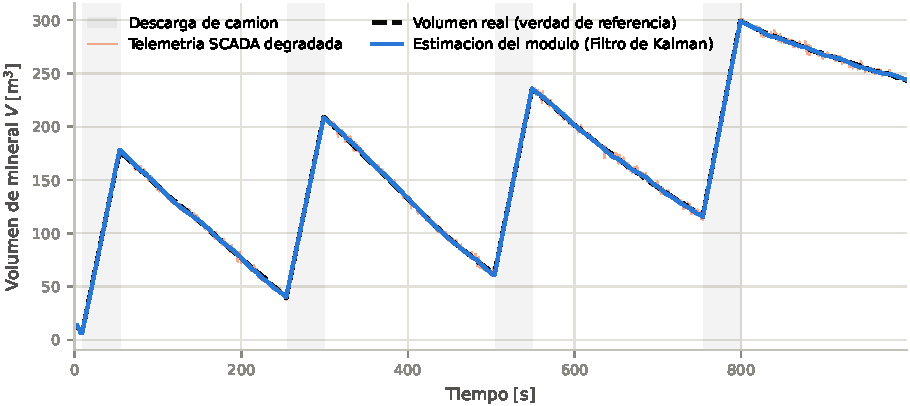
\includegraphics[width=\textwidth]{figuras/fig1_reconstruccion_volumen.pdf}
\caption{Reconstrucción dinámica del volumen de carga en la tolva de recepción.
Las bandas sombreadas indican los eventos de descarga de camión.}
\label{fig:reconstruccion}
\end{figure}

\subsection{Reconstrucción de la variable latente}

El resultado de mayor relevancia conceptual corresponde a la tasa de llenado
$\dot{V}_{k}$, variable que no cuenta con instrumentación alguna.

\begin{table}[H]
\centering
\caption{Métricas de error en la reconstrucción de la tasa de llenado, variable
no sensada.}
\label{tab:resultados-tasa}
\footnotesize
\begin{tabular}{@{}lS[table-format=1.4]S[table-format=1.4]S[table-format=2.2]@{}}
\toprule
\textbf{Métrica} & {\textbf{Diferencias finitas}} &
{\textbf{Filtro de Kalman}} & {\textbf{Reducción [\si{\percent}]}}\\
\midrule
RMSE [\si{\metre\cubed\per\second}] & 3.6891 & 0.0674 & 98.17\\
\bottomrule
\end{tabular}
\end{table}

La magnitud de la diferencia merece atención. La línea base disponible para un
sistema SCADA convencional —derivar numéricamente la señal cruda— produce un
error de \SI{3,69}{\metre\cubed\per\second} sobre una magnitud física cuyo valor
nominal es \SI{0,8}{\metre\cubed\per\second}: el procedimiento entrega ruido y
no información. El módulo reduce ese error a
\SI{0,067}{\metre\cubed\per\second}, lo que representa una mejora del
\SI{98,17}{\percent}. La figura~\ref{fig:latente} contrasta ambos
procedimientos.

\begin{figure}[H]
\centering
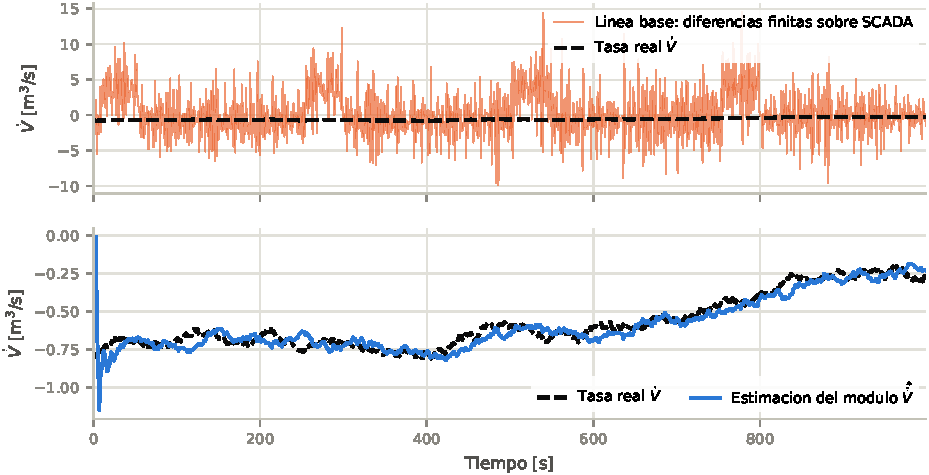
\includegraphics[width=\textwidth]{figuras/fig2_tasa_latente.pdf}
\caption{Recuperación de la variable latente. Panel superior: línea base por
diferencias finitas sobre la señal cruda. Panel inferior: estimación del módulo,
en escala física. Nótese la diferencia de escala entre ambos paneles.}
\label{fig:latente}
\end{figure}

\subsection{Convergencia asintótica del estimador}

La figura~\ref{fig:convergencia} evidencia la convergencia de la covarianza del
error y de la ganancia de Kalman hacia sus valores de régimen permanente,
comportamiento predicho por la formulación de Riccati para sistemas lineales
invariantes \parencite{simon2006}. La convergencia se alcanza en torno a los
\SI{60}{\second} de operación, con $K_{1} \to \num{0,0993}$.

\begin{figure}[H]
\centering
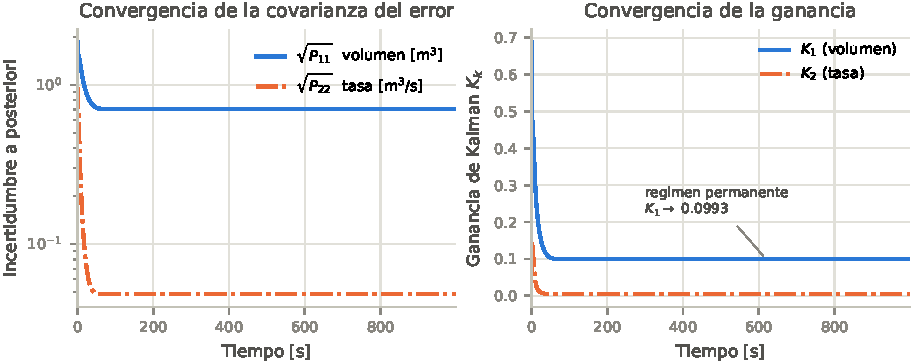
\includegraphics[width=\textwidth]{figuras/fig3_convergencia.pdf}
\caption{Convergencia asintótica de la covarianza del error de estimación y de
la ganancia de Kalman hacia el régimen permanente.}
\label{fig:convergencia}
\end{figure}

\subsection{Validación estadística}

La tabla~\ref{tab:inferencia} reporta la inferencia sobre el RMSE, expresada en
\si{\metre\cubed}.

\begin{table}[H]
\centering
\caption{Inferencia estadística pareada sobre el RMSE del volumen
($M = 50$; $\alpha = 0{,}05$).}
\label{tab:inferencia}
\footnotesize
\begin{tabular}{@{}ll@{}}
\toprule
\textbf{Estadístico} & \textbf{Valor}\\
\midrule
Reducción media del RMSE & \SI{1,5106}{\metre\cubed}\\
Intervalo de confianza al \SI{95}{\percent} &
$[1{,}4881;\ 1{,}5330]$~\si{\metre\cubed}\\
Prueba t pareada (unilateral) & $t(49) = 135{,}24$; $p = 5{,}15\times10^{-65}$\\
Tamaño del efecto ($d$ de Cohen) & \num{19,13}\\
Normalidad (Shapiro-Wilk) & $W = 0{,}9459$; $p = 0{,}0233$ \quad
\textbf{(se rechaza)}\\
Contraste robusto (Wilcoxon) & $W = 1275{,}0$; $p = 8{,}88\times10^{-16}$\\
Decisión & Se rechaza $H_{0}$\\
\bottomrule
\end{tabular}
\end{table}

Corresponde detenerse en el resultado de la verificación de normalidad. La
prueba de Shapiro-Wilk \textbf{rechaza} el supuesto de normalidad de las
diferencias ($p = 0{,}0233 < 0{,}05$), de modo que la aplicación mecánica de la
prueba t sería, en rigor, cuestionable. Es precisamente por esta razón que el
diseño incorporó el contraste no paramétrico de Wilcoxon, que no exige
normalidad y que confirma la conclusión con
$p = 8{,}88\times10^{-16}$. La coincidencia de ambas pruebas permite sostener el
rechazo de $H_{0}$ con independencia del supuesto paramétrico. Debe añadirse que
con $M = 50$ observaciones el teorema central del límite otorga a la prueba t
una robustez considerable frente a desviaciones moderadas de la normalidad, y
que la magnitud del efecto —una $d$ de Cohen de \num{19,13}, más de un orden de
magnitud por sobre el umbral convencional de efecto grande— hace que ninguna
consideración distribucional pueda revertir la conclusión.

Sobre la variable latente, la inferencia arroja $t(49) = 296{,}36$ con
$p = 1{,}09\times10^{-81}$ e intervalo de confianza al \SI{95}{\percent} de
$[3{,}5971;\ 3{,}6463]$~\si{\metre\cubed\per\second}.

\begin{figure}[H]
\centering
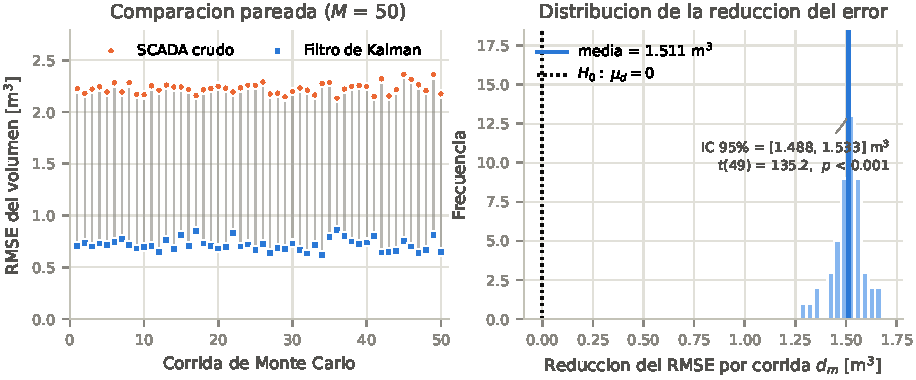
\includegraphics[width=\textwidth]{figuras/fig4_montecarlo.pdf}
\caption{Validación de Monte Carlo. Panel izquierdo: comparación pareada corrida
a corrida. Panel derecho: distribución de la reducción del RMSE, con la
hipótesis nula señalada en el origen.}
\label{fig:montecarlo}
\end{figure}

\subsection{Sensibilidad ante la degradación del entorno}

La tabla~\ref{tab:degradacion} y la figura~\ref{fig:degradacion} muestran el
comportamiento del módulo ante niveles crecientes de ruido real del sensor.

\begin{table}[H]
\centering
\caption{Desempeño del módulo ante niveles crecientes de degradación
instrumental.}
\label{tab:degradacion}
\footnotesize
\begin{tabular}{@{}S[table-format=3.0]S[table-format=2.2]S[table-format=3.3]S[table-format=2.3]S[table-format=2.2]@{}}
\toprule
{$R$ [\si{\metre\tothe{6}}]} & {$\sigma_{v}$ [\si{\metre\cubed}]} &
{MSE SCADA [\si{\metre\tothe{6}}]} & {MSE KF [\si{\metre\tothe{6}}]} &
{Reducción [\si{\percent}]}\\
\midrule
1   & 1.00  & 0.987   & 0.165  & 83.32\\
5   & 2.24  & 4.937   & 0.527  & 89.33\\
20  & 4.47  & 19.748  & 1.449  & 92.66\\
50  & 7.07  & 49.369  & 2.831  & 94.27\\
100 & 10.00 & 98.738  & 4.707  & 95.23\\
200 & 14.14 & 197.476 & 7.843  & 96.03\\
400 & 20.00 & 394.953 & 13.093 & 96.68\\
\bottomrule
\end{tabular}
\end{table}

La reducción del error crece de forma monótona con la severidad de la
degradación, desde el \SI{83,32}{\percent} en condiciones benignas hasta el
\SI{96,68}{\percent} en degradación extrema. El aporte del módulo, por tanto, no
se diluye en entornos hostiles sino que se acentúa.

\begin{figure}[H]
\centering
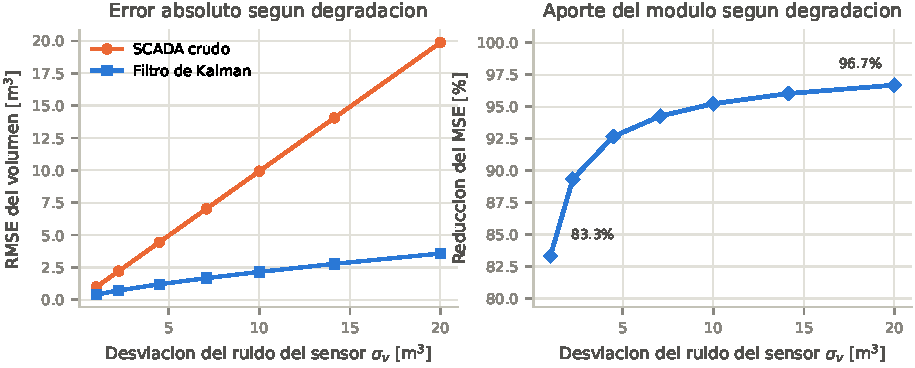
\includegraphics[width=\textwidth]{figuras/fig5_degradacion.pdf}
\caption{Comportamiento del módulo ante niveles crecientes de ruido
instrumental. Izquierda: error absoluto de ambas fuentes. Derecha: reducción
relativa del MSE.}
\label{fig:degradacion}
\end{figure}

\subsection{Robustez ante desajuste de sintonización}

La figura~\ref{fig:sensibilidad} presenta la malla de RMSE resultante de
desajustar intencionalmente las covarianzas del filtro respecto de la física
real.

\begin{figure}[H]
\centering
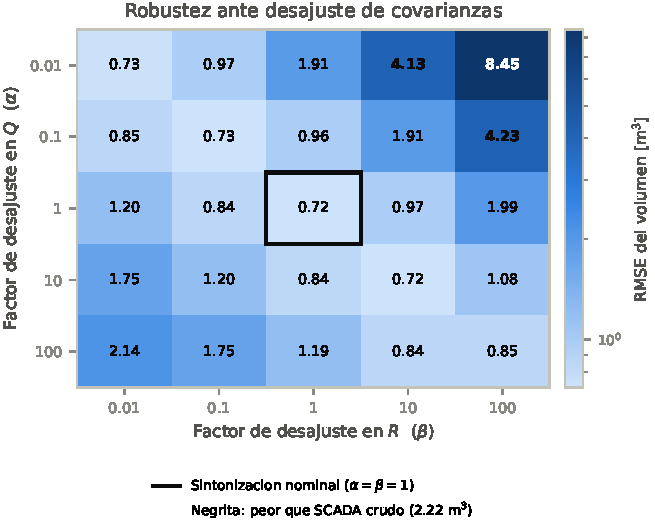
\includegraphics[width=0.82\textwidth]{figuras/fig6_sensibilidad_QR.pdf}
\caption{Robustez del módulo ante desajuste intencional de las covarianzas
$\mathbf{Q}$ y $\mathbf{R}$. El recuadro señala la sintonización nominal.}
\label{fig:sensibilidad}
\end{figure}

El resultado presenta una estructura diagonal marcada. Con sintonización nominal
el RMSE es \SI{0,721}{\metre\cubed}, frente a \SI{2,224}{\metre\cubed} de la
telemetría cruda. A lo largo de la diagonal —donde ambas covarianzas están
escaladas por el mismo factor, incluso hasta cien veces en cualquier dirección—
el desempeño se mantiene en el rango \SIrange{0,72}{0,85}{\metre\cubed}, muy
cerca del óptimo. La degradación severa aparece solo en las esquinas
antidiagonales, y el peor caso de la malla alcanza \SI{8,45}{\metre\cubed}.

De las veinticinco combinaciones evaluadas, únicamente tres resultan peores que
no filtrar. Este hallazgo tiene una lectura de ingeniería directa: lo que
gobierna el desempeño del estimador es la \emph{razón} $\mathbf{Q}/\mathbf{R}$ y
no los valores absolutos de ambas matrices, resultado consistente con la teoría
de estimación óptima y de considerable valor práctico, puesto que implica que un
error de calibración proporcional en ambas covarianzas es esencialmente
inofensivo.

\subsection{Verificación de reproducibilidad}

Dos ejecuciones sucesivas e independientes del experimento produjeron archivos
de salida idénticos byte a byte, verificado mediante suma de verificación MD5
sobre los cuatro registros CSV generados. La reproducibilidad exacta del estudio
es, por tanto, un hecho comprobado y no una declaración de intención.

\subsection{Extensibilidad del núcleo del módulo}
\label{sec:extensibilidad}

Como evidencia complementaria del carácter desacoplado del módulo, el mismo
núcleo del estimador se aplicó sin modificación alguna de su código a otros tres
subsistemas del activo: la dinámica electromecánica de potencia activa del motor
principal, la dinámica térmica del estator y la tendencia de desgaste
estructural del revestimiento. En los tres casos únicamente se sustituyen las
matrices del sistema que se entregan al constructor de la clase.

Este resultado no forma parte de la validación central del estudio, cuyo objeto
declarado es el volumen de tolva, pero acredita empíricamente la propiedad de
autocontención y desacoplamiento comprometida en el alcance del proyecto, y
sugiere una vía de extensión natural que se recoge en las proyecciones de la
sección~\ref{sec:conclusiones}.

\section{Criterios de calidad del estudio}
\label{sec:calidad}

El rigor científico y metodológico del estudio se verifica mediante cuatro
criterios, cada uno con su mecanismo concreto de control y su evidencia de
verificación.

\subsection{Validez interna y trazabilidad}

\textbf{Definición.} La capacidad de atribuir las diferencias observadas en el
error exclusivamente al módulo evaluado, y de que un tercero obtenga exactamente
las mismas salidas.

\textbf{Mecanismo.} Aislamiento del entorno de ejecución, fijación determinista
de la semilla del generador pseudoaleatorio, derivación de flujos aleatorios
independientes por corrida a partir de una única semilla maestra, y
parametrización centralizada en una estructura inmutable.

\textbf{Verificación.} Se ejecutó el experimento completo dos veces de forma
independiente y se compararon los cuatro archivos CSV generados mediante suma de
verificación MD5, obteniendo identidad byte a byte. Este criterio, que en las
entregas previas se declaraba sin demostración, se encuentra ahora comprobado.

\subsection{Confiabilidad y convergencia asintótica}

\textbf{Definición.} La estabilidad de las conclusiones frente a la
variabilidad estocástica inherente al proceso.

\textbf{Mecanismo.} Diseño de Monte Carlo con $M = 50$ corridas independientes
de $N = 1000$ pasos, que asegura la convergencia de la ganancia
$\mathbf{K}_{k}$ y de la covarianza $\mathbf{P}_{k|k}$ hacia sus valores de
régimen permanente según la formulación de Riccati.

\textbf{Verificación.} La figura~\ref{fig:convergencia} documenta la
convergencia efectiva de ambas magnitudes. La dispersión de las métricas entre
corridas es reducida —desviación estándar del RMSE de \SI{0,059}{\metre\cubed}
para el filtro— y la comparación pareada de la figura~\ref{fig:montecarlo}
muestra que la ventaja del módulo se sostiene en las cincuenta corridas sin
excepción.

\subsection{Validez de constructo}

\textbf{Definición.} La correspondencia entre el modelo matemático implementado
y el fenómeno físico que pretende representar.

\textbf{Mecanismo.} Las matrices del modelo se derivan estrictamente de la ley
de conservación de masa de la tolva, y no de un ajuste empírico a los datos. Los
parámetros dimensionales se calibran contra la escala real del activo: la tasa
de extracción corresponde a la capacidad documentada de un chancador giratorio
de gran minería, y el volumen por evento de descarga al tonelaje de un camión de
extracción, según se justifica en la tabla~\ref{tab:parametros}.

\textbf{Verificación.} Además de la trazabilidad física de cada parámetro, se
verifica computacionalmente la condición de observabilidad del par
$(\mathbf{A}, \mathbf{H})$ antes de cada corrida
(ecuación~\eqref{eq:observabilidad}), y se comprobó que el MSE de la telemetría
cruda coincide con la varianza de ruido inyectada, lo que confirma la
implementación correcta del generador de degradación.

Corresponde señalar aquí, como control de calidad efectivamente aplicado, que
este criterio condujo a la detección y corrección de la inconsistencia física de
la covarianza de proceso documentada en la sección~\ref{sec:recalibracion}.

\subsection{Sensibilidad y robustez}

\textbf{Definición.} Los márgenes dentro de los cuales el módulo conserva su
utilidad frente a variaciones del entorno y errores de calibración.

\textbf{Mecanismo.} Dos experimentos independientes: barrido de la varianza real
del sensor sobre dos órdenes de magnitud, y malla de desajuste intencional de
las razones de covarianza $\mathbf{Q}/\mathbf{R}$ sobre un rango de cuatro
órdenes de magnitud.

\textbf{Verificación.} Los resultados de las tablas~\ref{tab:degradacion} y de
la figura~\ref{fig:sensibilidad} acreditan que el aporte del módulo crece con la
degradación del entorno y que veintidós de veinticinco combinaciones de
sintonización superan a la línea base. Este criterio, declarado en el diseño
metodológico de la Fase 3, se implementa efectivamente en esta entrega.

\subsection{Limitaciones de los criterios de calidad}

La honestidad metodológica exige declarar el alcance de estos criterios. La
validez interna del estudio es alta, pero su \textbf{validez externa} está
acotada por construcción: los resultados acreditan el desempeño del estimador
sobre un proceso que satisface exactamente los supuestos del modelo —linealidad,
ruido gaussiano blanco, covarianzas conocidas—, condición que una planta real
solo cumple de manera aproximada. El análisis de robustez de la
sección~\ref{sec:resultados} mitiga parcialmente esta limitación al evaluar el
desempeño bajo desajuste de covarianzas, pero no sustituye la validación con
telemetría real, que queda declarada como trabajo futuro en la
sección~\ref{sec:conclusiones}.

\section{Consideraciones éticas}
\label{sec:etica}

El estudio no involucra participantes humanos ni datos personales, por lo que
los resguardos éticos no se orientan al consentimiento informado sino a la
responsabilidad profesional en el manejo de información industrial y en la
comunicación de resultados de ingeniería. Los resguardos se estructuran bajo el
esquema riesgo~$\rightarrow$~acción de mitigación.

\subsection{Riesgo 1: Sobreatribución de madurez tecnológica}

\textbf{Riesgo.} Presentar un modelo matemático validado exclusivamente sobre
datos sintéticos como si fuera un producto informático listo para sustentar
decisiones operativas reales en planta. Este es el riesgo central y más propio
de este estudio. Su materialización podría inducir falsas expectativas de
seguridad o de rendimiento industrial, y en un contexto donde las decisiones de
alimentación de un chancador tienen consecuencias sobre la integridad del equipo
y sobre la seguridad de las personas, esa sobreatribución no es un problema
meramente académico.

\textbf{Acción de mitigación.} Se declara de manera explícita, en el informe, en
el artículo científico y en la presentación oral, que el algoritmo propuesto se
encuentra en un nivel de madurez tecnológica de laboratorio y simulación. Se
exige de forma expresa el pilotaje físico \emph{in situ} y la calibración
empírica de seguridad como condiciones previas a cualquier despliegue comercial
en un gemelo digital operativo. Esta declaración se incorpora además al archivo
\texttt{README} del código entregado, de modo que acompañe al artefacto y no
solo al documento.

\subsection{Riesgo 2: Exposición de información industrial confidencial}

\textbf{Riesgo.} Vulnerar los acuerdos de no divulgación vigentes en la
industria minera mediante la exposición de telemetría propietaria, leyes de
mineral o rendimientos comerciales de faenas específicas.

\textbf{Acción de mitigación.} El proyecto prescinde por completo de datos
telemétricos crudos de yacimientos específicos y fundamenta su análisis en datos
sintéticos calibrados con literatura científica pública. Los parámetros
dimensionales utilizados corresponden a rangos genéricos de la gran minería a
cielo abierto documentados en fuentes abiertas, y no a valores de operación de
ninguna faena identificable. Con ello se anula el riesgo de filtración de
información estratégica.

\subsection{Riesgo 3: Integridad de los resultados reportados}

\textbf{Riesgo.} Reportar métricas de desempeño no verificables, ajustadas para
favorecer la conclusión, o no reproducibles por terceros.

\textbf{Acción de mitigación.} Se adopta un principio de reproducibilidad
estricta: todo valor numérico reportado en este informe proviene de la ejecución
del código anexo con semilla fija, y cualquier evaluador puede reejecutarlo y
obtener exactamente los mismos resultados. Se reportan tanto las métricas
favorables como las desfavorables —en particular, el rechazo del supuesto de
normalidad por la prueba de Shapiro-Wilk y las tres combinaciones de
sintonización en que el módulo resulta peor que no filtrar—, y se documentan de
forma explícita las recalibraciones de parámetros realizadas durante el
desarrollo, con su justificación física (sección~\ref{sec:recalibracion}).

\subsection{Riesgo 4: Trazabilidad y veracidad de las fuentes}

\textbf{Riesgo.} Sustentar afirmaciones del marco teórico o del estado del arte
en referencias no verificables, lo que comprometería la integridad académica del
trabajo y la validez de la brecha de conocimiento declarada.

\textbf{Acción de mitigación.} La totalidad de las referencias citadas fue
verificada individualmente contra su fuente primaria antes de la consolidación
de este informe. Se retiraron aquellas cuya existencia no pudo comprobarse y se
sustituyeron por fuentes verificadas de pertinencia equivalente o superior. Se
corrigió además la atribución editorial de una referencia que aparecía asignada
a una revista incorrecta en entregas previas. El Anexo~\ref{anexo:matriz}
consigna, para cada fuente, su identificador digital de objeto, lo que permite
la verificación independiente por parte del evaluador.

\subsection{Riesgo 5: Uso responsable de herramientas de asistencia}

\textbf{Riesgo.} Incorporar contenido generado por herramientas automatizadas
sin verificación, en particular datos, citas o resultados numéricos.

\textbf{Acción de mitigación.} Todo resultado numérico presentado procede de
código ejecutado y auditable, no de estimaciones. Toda referencia bibliográfica
fue contrastada con su fuente. El código, los registros de trazabilidad y las
figuras se entregan como anexo digital, de modo que la cadena completa entre el
dato y la afirmación sea inspeccionable.

\section{Coherencia metodológica del proyecto}
\label{sec:coherencia}

Esta sección analiza la coherencia interna del estudio, verificando que el
diseño metodológico efectivamente responde a la pregunta de investigación
formulada.

\subsection{Cadena de articulación}

El proyecto exhibe una articulación vertical unívoca. El \textbf{fenómeno}
—degradación estocástica de la telemetría en chancado primario— se delimita como
\textbf{problema} informático de observabilidad parcial; de ese problema se
deriva la \textbf{pregunta} sobre la capacidad de un estimador estocástico para
reconstruir el estado interno; la pregunta se descompone en cuatro
\textbf{objetivos} que cubren caracterización, modelación, implementación y
validación; y cada objetivo determina una \textbf{decisión metodológica} con su
instrumento correspondiente. La tabla~\ref{tab:coherencia} formaliza esa cadena
e incorpora la evidencia efectivamente producida.

\begin{table}[H]
\centering
\caption{Matriz de coherencia metodológica y trazabilidad del proyecto.}
\label{tab:coherencia}
\footnotesize
\begin{tabular}{@{}p{2.9cm}p{3.2cm}p{3.2cm}p{3.9cm}@{}}
\toprule
\textbf{Objetivo específico} & \textbf{Decisión metodológica} &
\textbf{Instrumento} & \textbf{Evidencia producida}\\
\midrule
\textbf{OE1.} Caracterizar el ruido SCADA en chancado primario &
Modelación de ruido gaussiano mediante $\mathbf{Q}$ y $\mathbf{R}$
parametrizadas &
Revisión de literatura indexada y generador de degradación &
Tabla~\ref{tab:parametros}; verificación de que
$\mathrm{MSE}_{\text{SCADA}} \approx R$\\
\addlinespace
\textbf{OE2.} Modelar la dinámica de flujo en la tolva &
Espacio de estados lineal en tiempo discreto con estado latente &
Ecuaciones de balance de masa y matrices
$\mathbf{A},\mathbf{B},\mathbf{H}$ &
Ecuaciones~\eqref{eq:vector-estado}--\eqref{eq:matrices};
observabilidad verificada, ec.~\eqref{eq:observabilidad}\\
\addlinespace
\textbf{OE3.} Desarrollar el Filtro de Kalman Lineal &
Programación modular científica con núcleo desacoplado &
Ciclo recursivo predictor-corrector en forma de Joseph &
Módulo ejecutable; figura~\ref{fig:convergencia};
sección~\ref{sec:extensibilidad}\\
\addlinespace
\textbf{OE4.} Validar el desempeño frente a la lectura degradada &
Monte Carlo e inferencia estadística pareada &
Métricas MSE/RMSE, prueba t, Wilcoxon y análisis de sensibilidad &
Tablas~\ref{tab:resultados-volumen}--\ref{tab:degradacion};
figuras~\ref{fig:montecarlo}--\ref{fig:sensibilidad}\\
\bottomrule
\end{tabular}
\end{table}

\subsection{Verificación de que el diseño responde a la pregunta}

La pregunta de investigación exige tres cosas y el diseño provee evidencia para
cada una.

Exige, primero, \textbf{mitigar el ruido instrumental}. El diseño lo verifica
comparando el error de la señal filtrada contra la línea base declarada, con una
verdad de referencia conocida por construcción, condición que solo la simulación
permite garantizar.

Exige, segundo, \textbf{reconstruir el estado dinámico interno} en un sistema
\textbf{parcialmente observable}. El diseño aborda esta exigencia de manera
directa mediante la incorporación de la tasa de llenado como estado latente no
sensado, y verifica formalmente la condición de observabilidad que hace posible
su reconstrucción. Sin ese segundo estado, el estudio no podría afirmar nada
sobre observabilidad parcial: se limitaría a suavizar una señal medida.

Exige, tercero, que la reconstrucción sea \textbf{confiable}. El diseño
operacionaliza esa exigencia mediante una prueba de hipótesis formal con nivel
de significancia declarado, un intervalo de confianza y un contraste de robustez
no paramétrico, de modo que la afirmación de confiabilidad sea verificable y no
argumentativa.

\subsection{Ajustes realizados para fortalecer la coherencia}

La coherencia del diseño no fue estática: se fortaleció mediante ajustes
concretos durante el desarrollo, la mayoría de ellos derivados de la
retroalimentación docente y documentados en el Anexo~\ref{anexo:ajustes}.

Tres de esos ajustes merecen mención en este análisis por su impacto en la
coherencia interna. El primero es la \textbf{separación dimensional} entre MSE y
RMSE, que resolvió la inconsistencia de reportar métricas en
\si{\metre\tothe{6}} junto a intervalos de confianza en \si{\metre\cubed}, y que
condujo a la decisión de fundar toda la inferencia sobre el RMSE. El segundo es
la \textbf{verificación empírica del supuesto de normalidad}, que reveló su
incumplimiento y motivó la incorporación del contraste de Wilcoxon; sin ese
ajuste, la conclusión estadística habría descansado sobre un supuesto no
satisfecho. El tercero es la \textbf{recalibración de la covarianza de proceso}
descrita en la sección~\ref{sec:recalibracion}, que restituyó la
correspondencia entre el modelo y la física del activo.

Corresponde señalar que los dos primeros ajustes fueron sugeridos por la
retroalimentación docente antes de que sus consecuencias fueran evidentes, y el
tercero emergió de la implementación efectiva del modelo. Esto ilustra que la
coherencia metodológica se verifica al construir, y no solo al declarar.

\section{Discusión}
\label{sec:discusion}

\subsection{Interpretación de los resultados frente a los objetivos}

Los resultados obtenidos permiten evaluar el cumplimiento de cada objetivo
específico y, por agregación, responder la pregunta de investigación.

Respecto de \textbf{OE1}, la caracterización del ruido se materializó en
matrices de covarianza con unidades explícitas y fundamento físico trazable, y
su corrección quedó verificada por la coincidencia entre el error de la
telemetría cruda y la varianza inyectada. Respecto de \textbf{OE2}, el modelo en
espacio de estados no solo se formuló sino que se sometió a una prueba
estructural: la verificación de observabilidad del par
$(\mathbf{A}, \mathbf{H})$, que constituye la condición matemática que habilita
todo lo demás. Respecto de \textbf{OE3}, el módulo se implementó como
componente desacoplado y su corrección numérica se verificó mediante la
convergencia de la ganancia y la covarianza hacia el régimen permanente.
Respecto de \textbf{OE4}, la validación arrojó una reducción del MSE del
\SI{89,57}{\percent}, estadísticamente significativa y robusta al supuesto
distribucional.

La respuesta a la pregunta de investigación es, por tanto, afirmativa en el
alcance declarado: el diseño y la validación mediante simulación estocástica de
un módulo basado en el Filtro de Kalman Lineal permiten mitigar el ruido
instrumental y reconstruir de forma confiable el estado dinámico interno de
volumen. Ahora bien, el significado de esa respuesta requiere ser interpretado
con precisión, y a ello se dedican los apartados siguientes.

\subsection{El hallazgo central: la variable que nadie mide}

El resultado de mayor densidad conceptual no es la reducción del error sobre el
volumen sino la reconstrucción de la tasa de llenado. La distinción importa.

Sobre el volumen, el módulo mejora una señal que \emph{ya existe}: hay un sensor
que la mide, y el filtro reduce su varianza. Es una contribución valiosa pero
incremental. Sobre la tasa de llenado, en cambio, el módulo produce información
que \emph{no existía en ninguna parte del sistema}. Ningún instrumento la mide,
y el único procedimiento disponible para un SCADA convencional —la derivada
numérica de la señal cruda— entrega un error de
\SI{3,69}{\metre\cubed\per\second} sobre una magnitud cuyo valor nominal es
\SI{0,8}{\metre\cubed\per\second}. Es decir, no entrega una estimación
imprecisa: entrega ruido con la apariencia de una medición.

Que el módulo reduzca ese error a \SI{0,067}{\metre\cubed\per\second} significa
que la capa analítica no está limpiando datos sino \emph{creando observabilidad}
donde la instrumentación no la provee. Esta es la evidencia empírica más directa
de la tesis del proyecto, y es también el argumento más fuerte a favor de
concebir el estimador como componente arquitectónico y no como filtro de
preprocesamiento: un preprocesador mejora lo que recibe, mientras que este
módulo entrega a las capas superiores una variable de estado que antes no
estaba disponible para la decisión.

\subsection{Contraste con la literatura}

Los hallazgos dialogan con los tres cuerpos de literatura revisados.

Frente a la literatura de \textbf{gemelos digitales}, los resultados dan
sustento cuantitativo a la distinción conceptual de \textcite{sepasgozar2021}
entre sombra digital y gemelo digital. Si la telemetría cruda de la tasa de
llenado es esencialmente ruido, una réplica virtual alimentada directamente por
el SCADA no está representando el activo sino su distorsión. La diferencia entre
ambos conceptos deja de ser terminológica y adquiere una magnitud medible.

Frente a la literatura de \textbf{gemelos digitales mineros}, el estudio se
alinea con el diagnóstico de \textcite{ebad2026} sobre la escasa validación
industrial del área y sobre la persistencia de los problemas de integración de
datos, y con la constatación de \textcite{qu2023} sobre la adopción fragmentada
en la industria de minerales. El aporte del proyecto consiste en atender
precisamente la capa que ambas revisiones señalan como desatendida: no la
sofisticación del modelo predictivo, sino la garantía de consistencia de sus
entradas.

Frente a la literatura de \textbf{estimación de estados en procesamiento de
minerales}, los resultados son consistentes con lo reportado por
\textcite{apelt2002} en molienda semiautógena y por \textcite{barzaga2025} en
lixiviación de cobre: variables internas no instrumentadas de procesos mineros
son efectivamente reconstruibles mediante estimación de estados. La diferencia
del presente trabajo respecto de ambos no es de resultado sino de encuadre.
Aquellos estudios formulan la estimación como instrumento de medición
inferencial o de control de procesos; este la formula como componente de una
arquitectura de gemelo digital, con las exigencias de desacoplamiento,
reproducibilidad y validación estadística que ese encuadre impone.

Cabe señalar que \textcite{barzaga2025} emplean variantes no lineales —filtros
extendido y \emph{unscented}— mientras que este proyecto se restringe
deliberadamente al caso lineal. Esa restricción no es una limitación
metodológica encubierta sino una decisión de alcance: el balance de masa de una
tolva es genuinamente lineal en el rango operacional considerado, y emplear un
estimador no lineal sobre un sistema lineal añadiría costo computacional sin
ganancia de precisión.

\subsection{El hallazgo sobre robustez y su implicancia práctica}

El análisis de sensibilidad produjo un resultado que no estaba previsto en el
plan original y que tiene consecuencias prácticas relevantes. La estructura
diagonal de la malla de desajuste muestra que el desempeño del estimador está
gobernado por la \emph{razón} entre las covarianzas y no por sus valores
absolutos: un error de calibración de dos órdenes de magnitud en ambas matrices
simultáneamente degrada el RMSE desde \num{0,72} hasta apenas
\SI{0,85}{\metre\cubed}, mientras que el mismo error aplicado a una sola de
ellas lo eleva hasta \SI{8,45}{\metre\cubed}.

La implicancia para una eventual implementación industrial es directa. La
dificultad práctica de sintonizar un filtro de Kalman en planta no reside en
determinar los valores absolutos de $\mathbf{Q}$ y $\mathbf{R}$ —tarea que
requeriría caracterización metrológica detallada— sino en estimar correctamente
su proporción, es decir, cuánto confiar en el modelo físico respecto del sensor.
Esta es una tarea considerablemente más accesible para un ingeniero de procesos,
y reduce la barrera de adopción del módulo.

El resultado del barrido de degradación apunta en la misma dirección: el aporte
del módulo crece con la hostilidad del entorno, desde el
\SI{83,32}{\percent} en condiciones benignas hasta el \SI{96,68}{\percent} en
degradación extrema. Cuanto peor es el entorno minero, más necesario resulta el
componente, lo que refuerza la pertinencia contextual del proyecto.

\subsection{Limitaciones del estudio}

La interpretación de los resultados exige declarar con precisión sus límites.

La limitación principal es que la validación se realiza sobre \textbf{datos
sintéticos generados por el mismo modelo que el filtro utiliza}. Bajo esa
condición, el Filtro de Kalman es el estimador óptimo por construcción teórica,
de modo que el estudio verifica la correcta implementación y cuantifica la
magnitud de la mejora, pero no somete al estimador a una discrepancia de modelo
genuina. El análisis de desajuste de covarianzas mitiga parcialmente esta
objeción, pero no la elimina: un proceso real puede presentar no linealidades,
ruido correlacionado o de color, y derivas no modeladas que este diseño no
reproduce.

La segunda limitación es de \textbf{alcance del modelo físico}. El balance de
masa implementado es una simplificación: no incorpora la geometría real de la
cámara, la segregación granulométrica del material, ni la dependencia de la tasa
de extracción respecto de la dureza instantánea del mineral. Se excluyeron
además los estados transitorios de arranque y parada y los eventos de
atascamiento, que son precisamente las condiciones de mayor interés operacional.

La tercera limitación es la \textbf{ausencia de validación con telemetría
real}, consecuencia directa de las restricciones de confidencialidad
documentadas. Esto sitúa el trabajo en un nivel de madurez tecnológica de
laboratorio y simulación, y ninguna de las cifras reportadas puede interpretarse
como una predicción del desempeño en planta.

Una cuarta consideración, de orden estadístico, es que el rechazo del supuesto
de normalidad por la prueba de Shapiro-Wilk, si bien queda cubierto por el
contraste de Wilcoxon, sugiere que la distribución de las diferencias presenta
una estructura que este estudio no exploró en profundidad y que podría ser
objeto de análisis posterior.

\subsection{Implicancias y proyecciones}

Pese a las limitaciones declaradas, el estudio sostiene una afirmación que
excede su caso particular: en arquitecturas de inteligencia artificial
industrial, la capa de consistencia física de los datos no es una etapa de
preprocesamiento sino un componente de diseño de primer orden, y su ausencia
compromete la validez de todo lo que se construya encima.

La evidencia de extensibilidad del núcleo del módulo reportada en la
sección~\ref{sec:extensibilidad}, donde el mismo estimador opera sin
modificación sobre potencia, temperatura y desgaste, sugiere que esta capa puede
concebirse como un servicio transversal del gemelo digital antes que como una
solución puntual por variable, línea que se recoge en las proyecciones del
estudio.

\section{Conclusiones}
\label{sec:conclusiones}

\subsection{Síntesis de los hallazgos}

El proyecto diseñó, implementó y validó estadísticamente un módulo de software
analítico basado en el Filtro de Kalman Lineal Discreto, concebido como capa de
consistencia física entre la telemetría degradada de un chancador primario y las
capas superiores de decisión de un gemelo digital.

Sobre la variable observada, el módulo redujo el error cuadrático medio del
volumen de carga en un \SI{89,57}{\percent} respecto de la lectura SCADA cruda,
reducción estadísticamente significativa según prueba t pareada
($t(49) = 135{,}24$; $p < 0{,}001$) y confirmada por contraste no paramétrico de
Wilcoxon ante el rechazo del supuesto de normalidad. Sobre la variable latente
—la tasa de llenado, que ningún instrumento mide— el módulo redujo el error en
un \SI{98,17}{\percent} respecto del único procedimiento disponible para un
SCADA convencional, produciendo información de estado que antes no existía en el
sistema.

El análisis de sensibilidad acreditó que el aporte del módulo crece con la
degradación del entorno, y que su desempeño está gobernado por la razón entre
las covarianzas de proceso y medición antes que por sus valores absolutos,
hallazgo que reduce sustantivamente la dificultad práctica de sintonización.

\subsection{Cumplimiento de los objetivos}

Los cuatro objetivos específicos se cumplieron, y cada uno generó el entregable
auditable comprometido en el plan del proyecto: matrices de covarianza
parametrizadas con fundamento físico trazable (OE1), un modelo en espacio de
estados con observabilidad verificada formalmente (OE2), un módulo de software
operativo, desacoplado y reproducible (OE3), y una validación estadística
completa con análisis de robustez (OE4). El objetivo general —diseñar y validar
mediante simulación estocástica el módulo, optimizando la observabilidad y
reduciendo el error cuadrático medio— se alcanzó dentro del alcance declarado.

\subsection{Aportes del estudio}

El aporte del trabajo no reside en el algoritmo, que es teoría establecida desde
\textcite{kalman1960}, sino en tres planos distintos.

En el plano \textbf{arquitectónico}, el estudio formula la estimación estocástica
de estados como componente de diseño de un gemelo digital minero, y no como
instrumento de control ni como etapa de preprocesamiento, atendiendo la capa que
las revisiones de \textcite{qu2023} y \textcite{ebad2026} identifican como
desatendida.

En el plano \textbf{empírico}, aporta evidencia cuantificada de que la
diferencia entre una sombra digital y un gemelo digital es medible, y de que la
capa analítica puede generar observabilidad allí donde la instrumentación no la
provee.

En el plano \textbf{metodológico}, entrega un artefacto reproducible byte a
byte, con registros de trazabilidad, verificación de supuestos estadísticos y
análisis de robustez paramétrica, en un área donde la validación efectiva ha sido
señalada como carencia.

\subsection{Recomendaciones y líneas de continuidad}

Se identifican cuatro líneas de continuidad, ordenadas por proximidad.

La primera y más inmediata es la \textbf{validación con telemetría real} de una
faena operativa, que permitiría contrastar el desempeño bajo discrepancia
genuina de modelo y determinar el nivel de madurez tecnológica efectivamente
alcanzable. Esta línea es condición necesaria para cualquier despliegue.

La segunda es la \textbf{extensión a regímenes no lineales}, incorporando los
estados transitorios de arranque y parada y los eventos de atascamiento que este
estudio excluyó, lo que requeriría migrar hacia variantes extendida o
\emph{unscented} del estimador, siguiendo el camino de \textcite{barzaga2025}.

La tercera es la \textbf{sintonización adaptativa} de las covarianzas, sugerida
directamente por el hallazgo sobre la razón $\mathbf{Q}/\mathbf{R}$: un
mecanismo que ajuste esa proporción en línea a partir de la secuencia de
innovaciones reduciría aún más la barrera de adopción industrial.

La cuarta es la \textbf{generalización del módulo como servicio transversal} del
gemelo digital, aplicando el mismo núcleo a los distintos subsistemas del activo
según la evidencia de extensibilidad reportada en la
sección~\ref{sec:extensibilidad}.

\subsection{Reflexión final}

La afirmación que sostiene este proyecto es que la inteligencia artificial
industrial requiere obligatoriamente limpiar matemáticamente sus datos antes de
tomar decisiones operacionales. Los resultados obtenidos permiten precisarla:
no se trata solo de limpiar, sino de \emph{reconstruir}. En un sistema
parcialmente observable, la capa de consistencia física no mejora la información
disponible, sino que produce información que la instrumentación no puede
entregar. Reconocer esa función es lo que justifica tratarla como componente
arquitectónico de primer orden y no como un accesorio del \emph{pipeline} de
datos.


% =============================================================================
%  REFERENCIAS
% =============================================================================
\newpage
{\singlespacing
\printbibliography[title={Referencias}]
}
\addcontentsline{toc}{section}{Referencias}

% =============================================================================
%  ANEXOS
% =============================================================================
\newpage
\appendix
\section*{Anexos}
\addcontentsline{toc}{section}{Anexos}
\renewcommand{\thesubsection}{\Alph{subsection}}
\setcounter{subsection}{0}

% =============================================================================
\subsection{Matriz de revisión bibliográfica}
\label{anexo:matriz}

La tabla~\ref{tab:matriz-biblio} sistematiza las fuentes utilizadas. Todas
fueron verificadas individualmente contra su fuente primaria en septiembre de
2026; se consigna el identificador digital de objeto de cada una para permitir
la verificación independiente por parte del evaluador.

\begin{table}[H]
\centering
\caption{Matriz de revisión bibliográfica.}
\label{tab:matriz-biblio}
\scriptsize
\begin{tabular}{@{}p{2.4cm}p{1.5cm}p{3.1cm}p{3.4cm}p{3.3cm}@{}}
\toprule
\textbf{Fuente} & \textbf{Eje} & \textbf{Aporte principal} &
\textbf{Relación con el proyecto} & \textbf{DOI}\\
\midrule
\textcite{kalman1960} & Estimación &
Estimador recursivo de varianza mínima para sistemas lineales &
Fundamento algorítmico del módulo (OE3) &
10.1115/1.3662552\\
\addlinespace
\textcite{simon2006} & Estimación &
Tratamiento moderno de la estimación óptima y convergencia de Riccati &
Sustento de la convergencia asintótica (OE3, OE4) &
10.1002/0470045345\\
\addlinespace
\textcite{lee2008} & Gemelos &
Formulación del paradigma de sistemas ciberfísicos &
Encuadre del acoplamiento físico-computacional &
10.1109/ISORC.2008.25\\
\addlinespace
\textcite{uhlemann2017} & Gemelos &
Gemelo digital como realización del sistema ciberfísico &
Contrapunto: sitúa la brecha en el \emph{middleware} &
10.1016/j.procir.2016.11.152\\
\addlinespace
\textcite{tao2019} & Gemelos &
Gemelo digital para pronóstico y gestión de salud de equipos &
Aplicación industrial de referencia; asume telemetría limpia &
10.1016/j.cirp.2019.04.049\\
\addlinespace
\textcite{fuller2020} & Gemelos &
Tecnologías habilitantes y desafíos abiertos &
Reconoce la calidad de datos como problema no resuelto &
10.1109/ACCESS.2020.2998358\\
\addlinespace
\textcite{liu2021} & Gemelos &
Revisión de conceptos, tecnologías y aplicaciones industriales &
Estado de adopción industrial del paradigma &
10.1016/j.jmsy.2020.06.017\\
\addlinespace
\textcite{sepasgozar2021} & Gemelos &
Distinción entre sombra digital y gemelo digital &
Criterio conceptual central del proyecto &
10.3390/buildings11040151\\
\addlinespace
\textcite{apelt2002} & Minería &
Medición inferencial de parámetros de molino SAG por estimación de estados &
Precedente directo de reconstrucción de estados en conminución &
10.1016/S0892-6875(02)00229-7\\
\addlinespace
\textcite{qu2023} & Minería &
Revisión comprehensiva de gemelos digitales en la industria de minerales &
Evidencia de adopción fragmentada; sitúa el vacío &
10.1080/25726668.2023.2257479\\
\addlinespace
\textcite{barzaga2025} & Minería &
Filtros de Kalman extendido y \emph{unscented} en lixiviación de cobre &
Precedente en minería del cobre; contraste lineal / no lineal &
10.3390/min15050521\\
\addlinespace
\textcite{ebad2026} & Minería &
Revisión sistemática de 68 estudios de gemelos digitales con IA en minería &
Documenta la escasa validación industrial: sustenta el vacío &
10.3390/technologies14050269\\
\bottomrule
\end{tabular}
\end{table}

\subsubsection*{Nota sobre depuración bibliográfica}

Durante la consolidación de esta entrega se verificó la totalidad de las
referencias empleadas en las fases previas. Cuatro de ellas no pudieron ser
localizadas en sus revistas de origen ni en repositorios bibliográficos, por lo
que fueron retiradas del trabajo y sustituidas por fuentes verificadas de
pertinencia equivalente o superior. Adicionalmente, se corrigió la atribución
editorial de \textcite{sepasgozar2021}, que en entregas anteriores aparecía
asignada a una revista distinta de aquella en que fue efectivamente publicada.
Esta depuración se documenta aquí en cumplimiento del principio de integridad
académica declarado en la sección~\ref{sec:etica}.

% =============================================================================
\subsection{Matriz de correspondencia entre el informe y el artículo científico}
\label{anexo:correspondencia}

\begin{table}[H]
\centering
\caption{Correspondencia entre secciones del informe final y del artículo
científico en formato IEEE.}
\label{tab:correspondencia}
\footnotesize
\begin{tabular}{@{}p{4.6cm}p{4.6cm}p{4.2cm}@{}}
\toprule
\textbf{Sección del informe} & \textbf{Sección del artículo} &
\textbf{Estado de trazabilidad}\\
\midrule
\S\ref{sec:fenomeno}--\ref{sec:pregunta} Fenómeno, problema y pregunta &
I. Introduction & Consolidado\\
\addlinespace
\S\ref{sec:estado-arte} Estado del arte y vacío &
II. Related Work & Consolidado; misma bibliografía verificada\\
\addlinespace
\S\ref{sec:unidad} Unidad de análisis &
III. Problem Formulation & Modelo y matrices unificados\\
\addlinespace
\S\ref{sec:enfoque}--\ref{sec:procedimientos} Metodología &
IV. Methodology & Consolidado\\
\addlinespace
\S\ref{sec:analisis} Estrategia de análisis &
IV.D. Evaluation Metrics and Tests & Métricas y pruebas unificadas\\
\addlinespace
\S\ref{sec:resultados} Resultados &
V. Results & Mismas figuras y valores numéricos\\
\addlinespace
\S\ref{sec:discusion} Discusión &
VI. Discussion & Consolidado\\
\addlinespace
\S\ref{sec:conclusiones} Conclusiones &
VII. Conclusion & Consolidado\\
\bottomrule
\end{tabular}
\end{table}

La trazabilidad entre ambos productos es verificable y no meramente declarada:
comparten el mismo archivo de referencias, las mismas figuras generadas por el
código anexo y los mismos valores numéricos, de modo que cualquier discrepancia
sería detectable por inspección directa.

% =============================================================================
\subsection{Ajustes derivados de la retroalimentación docente}
\label{anexo:ajustes}

\begin{table}[H]
\centering
\caption{Registro de ajustes incorporados en la entrega final.}
\label{tab:ajustes}
\footnotesize
\begin{tabular}{@{}p{1.8cm}p{4.6cm}p{4.6cm}p{2.4cm}@{}}
\toprule
\textbf{Origen} & \textbf{Observación recibida} & \textbf{Ajuste realizado} &
\textbf{Sección}\\
\midrule
Fases 1--3 &
Lista de referencias en formato numérico cuando la pauta exige APA 7
autor-fecha &
Unificación completa bajo APA 7 mediante gestor bibliográfico &
Referencias\\
\addlinespace
Fase 1 &
Ausencia de matriz de revisión bibliográfica &
Incorporación de la matriz con caracterización y DOI de cada fuente &
Anexo~\ref{anexo:matriz}\\
\addlinespace
Fase 1 &
El plan del proyecto era en realidad una sección de alcances; faltaban
resultados esperados, hitos, avances ABP y trazabilidad al artículo &
Formulación completa del plan con etapas, entregables, indicadores, hitos,
criterios de seguimiento y viabilidad &
\S\ref{sec:plan}\\
\addlinespace
Fase 1 &
Cita de un \emph{working paper} propio no publicado como respaldo externo &
Retirada; sustituida por fuentes indexadas verificadas &
Anexo~\ref{anexo:matriz}\\
\addlinespace
Fase 2 &
Trazabilidad con el artículo declarada pero no verificable &
Matriz de correspondencia explícita y recursos compartidos entre ambos
productos &
Anexo~\ref{anexo:correspondencia}\\
\addlinespace
Fase 2 &
Enunciar los objetivos específicos y amarrarlos a cada eje conceptual del marco
teórico &
Cada eje del marco teórico declara explícitamente el objetivo que sustenta &
\S\ref{sec:marco}\\
\addlinespace
Fase 3 &
Consideraciones éticas sin estructura riesgo--mitigación y sin nombrar el riesgo
central del estudio &
Reestructuración en cinco riesgos con su acción de mitigación, encabezados por
la sobreatribución de madurez tecnológica &
\S\ref{sec:etica}\\
\addlinespace
Fase 3 &
Revisar la unidad de la varianza $R$ &
Declaración explícita de unidades de todos los parámetros con su fundamento
físico &
Tabla~\ref{tab:parametros}\\
\addlinespace
Fase 3 &
Verificar el supuesto de normalidad de la prueba t &
Prueba de Shapiro-Wilk aplicada; ante su rechazo se incorporó el contraste no
paramétrico de Wilcoxon &
\S\ref{sec:analisis}, \S\ref{sec:resultados}\\
\addlinespace
Fase 3 &
Incoherencia dimensional: MSE en \si{\metre\tothe{6}} e intervalo de confianza
en \si{\metre\cubed} &
Separación explícita de métricas; toda la inferencia se funda sobre el RMSE en
\si{\metre\cubed} &
\S\ref{sec:analisis}\\
\addlinespace
Fase 3 &
Unificación del título del artículo científico &
Título del artículo alineado con el foco en chancado primario &
Artículo IEEE\\
\addlinespace
Fase 3 &
Análisis de sensibilidad declarado en los criterios de calidad pero no
ejecutado &
Implementación del barrido de degradación y de la malla de desajuste
$\mathbf{Q}/\mathbf{R}$ &
\S\ref{sec:resultados}\\
\bottomrule
\end{tabular}
\end{table}

Se incorporaron además dos ajustes que no provienen de la retroalimentación sino
de la implementación efectiva del modelo: la recalibración de la covarianza de
proceso $Q_{22}$ por implausibilidad física
(\S\ref{sec:recalibracion}) y la unificación de la condición inicial del
sistema, que presentaba valores distintos en documentos previos.

% =============================================================================
\subsection{Anexo digital: código fuente y registros de trazabilidad}
\label{anexo:codigo}

Se adjunta el paquete completo del módulo, cuya estructura es la siguiente:

\begin{table}[H]
\centering
\caption{Contenido del anexo digital.}
\label{tab:anexo-digital}
\footnotesize
\begin{tabular}{@{}p{4.6cm}p{8.6cm}@{}}
\toprule
\textbf{Componente} & \textbf{Descripción}\\
\midrule
\texttt{nucleo\_kalman.py} &
Núcleo del estimador, genérico y desacoplado del proceso físico\\
\texttt{modelo\_tolva.py} &
Modelo de referencia de la tolva, parametrización y degradación SCADA\\
\texttt{analisis.py} &
Métricas de error, simulación de Monte Carlo e inferencia estadística\\
\texttt{sensibilidad.py} &
Barrido de degradación y malla de desajuste de covarianzas\\
\texttt{figuras.py} &
Generación de las figuras del informe y del artículo\\
\texttt{main.py} &
Punto de entrada único del experimento\\
\texttt{README.md} &
Documentación, parametrización y declaración de madurez tecnológica\\
\texttt{resultados/logs/} &
Cuatro registros CSV de trazabilidad\\
\texttt{resultados/figuras/} &
Seis figuras en formato vectorial y de mapa de bits\\
\texttt{resultados/resultados.json} &
Parametrización, entorno de ejecución y resumen consolidado\\
\bottomrule
\end{tabular}
\end{table}

La ejecución del archivo \texttt{main.py} en un entorno con Python~3, NumPy,
SciPy y Matplotlib reproduce la totalidad de los resultados reportados en este
informe.


\end{document}
